%%%%%%%%%%%%%%%%%%%%%%%%%%%%%%%%%%%%%%%%%
% Beamer Presentation
% LaTeX Template
% Version 1.0 (10/11/12)
%
% This template has been downloaded from:
% http://www.LaTeXTemplates.com
%
% License:
% CC BY-NC-SA 3.0 (http://creativecommons.org/licenses/by-nc-sa/3.0/)
%
%%%%%%%%%%%%%%%%%%%%%%%%%%%%


%----------------------------------------------------------------------------------------
%	PACKAGES AND THEMES
%----------------------------------------------------------------------------------------

%\documentclass[10pt]{beamer}
\documentclass[aspectratio=169]{beamer}



\DeclareMathOperator*{\argmin}{arg\,min}


%%%%%%%%%%%%%

\usepackage{hyperref}


\newcommand{\bi}{\begin{itemize}}
\newcommand{\ei}{\end{itemize}}
\newcommand{\m}{\item}
\newcommand{\be}{\begin{enumerate}}
\newcommand{\ee}{\end{enumerate}}
\newcommand{\al}{\alert}
\newcommand{\ul}{\underline}


\mode<presentation> {

% The Beamer class comes with a number of default slide themes
% which change the colors and layouts of slides. Below this is a list
% of all the themes, uncomment each in turn to see what they look like.

%\usetheme{default}
%\usetheme{AnnArbor}
%\usetheme{Antibes}
%\usetheme{Bergen}
%\usetheme{Berkeley}
%\usetheme{Berlin}
%\usetheme{Boadilla}
%\usetheme{CambridgeUS}
%\usetheme{Copenhagen}
%\usetheme{Darmstadt}
%\usetheme{Dresden}
\usetheme{Frankfurt}
%\usetheme{Goettingen}
%\usetheme{Hannover}
%\usetheme{Ilmenau}
%\usetheme{JuanLesPins}
%\usetheme{Luebeck}
%\usetheme{Madrid}
%\usetheme{Malmoe}
%\usetheme{Marburg}
%\usetheme{Montpellier}
%\usetheme{PaloAlto}
%\usetheme{Pittsburgh}
%\usetheme{Rochester}
%\usetheme{Singapore}
%\usetheme{Szeged}
%\usetheme{Warsaw}

% As well as themes, the Beamer class has a number of color themes
% for any slide theme. Uncomment each of these in turn to see how it
% changes the colors of your current slide theme.

%\usecolortheme{albatross}
%\usecolortheme{beaver}
%\usecolortheme{beetle}
%\usecolortheme{crane}
%\usecolortheme{dolphin}
%\usecolortheme{dove}
%\usecolortheme{fly}
%\usecolortheme{lily}
%\usecolortheme{orchid}
%\usecolortheme{rose}
%\usecolortheme{seagull}
%\usecolortheme{seahorse}
%\usecolortheme{whale}
%\usecolortheme{wolverine}

%\setbeamertemplate{footline} % To remove the footer line in all slides uncomment this line
%\setbeamertemplate{footline}[page number] % To replace the footer line in all slides with a simple slide count uncomment this line

%\setbeamertemplate{navigation symbols}{} % To remove the navigation symbols from the bottom of all slides uncomment this line
}


%\setbeamertemplate{headline}
%{%
% \begin{beamercolorbox}{section in head/foot}
%\vskip1pt\insertnavigation{\textwidth}{}{}\vskip2pt
%  \end{beamercolorbox}
%}


%---------------------------------------------------------------
%---------------------------------------------------------------
%------------- beginning: global frame setting -----------
\usepackage[dvipsnames]{xcolor}

\setbeamercolor{frametitle}{bg=NavyBlue}
\setbeamercolor{section in head/foot}{fg=blue,bg=white} %set the top navigation bar background color
\setbeamertemplate{footline}[frame number] % set frame page number only
\usepackage{appendixnumberbeamer} % total will not include appendix frame numbers 

% the following line hide the beamer navigation symbols
\beamertemplatenavigationsymbolsempty

% https://tex.stackexchange.com/questions/83048/change-the-contents-of-footline-in-a-beamer-presentation
\setbeamertemplate{footline}
{
  \leavevmode%
  \hbox{%
  \begin{beamercolorbox}[wd=.3\paperwidth,ht=2.25ex,dp=1ex,center]{author in head/foot}%
    \usebeamerfont{author in head/foot}\insertshortinstitute
  \end{beamercolorbox}%
  \begin{beamercolorbox}[wd=.4\paperwidth,ht=2.25ex,dp=1ex,center]{title in head/foot}%
    \usebeamerfont{title in head/foot}\insertshorttitle
  \end{beamercolorbox}%
  \begin{beamercolorbox}[wd=.3\paperwidth,ht=2.25ex,dp=1ex,right]{date in head/foot}%
    \usebeamerfont{date in head/foot}\hspace*{4em} \insertshortauthor \hspace*{4em}
    \insertframenumber{} / \inserttotalframenumber\hspace*{2ex} 
  \end{beamercolorbox}}%
  \vskip0pt%
}

\setbeamercolor{author in head/foot}{bg=NavyBlue}
\setbeamercolor{title in head/foot}{bg=Gray}
\setbeamercolor{date in head/foot}{bg=NavyBlue}

%------------- ending: global frame setting -----------
%---------------------------------------------------------------
%---------------------------------------------------------------



\usepackage{graphicx} % Allows including images
% graphicx also allows for resizebox
% graphicx also allows for \scalebox
\usepackage{caption}
\usepackage{subcaption} % packgage for subcaption in subfigures
% The subfig and subcaption packages can not be used in cooperation with each other. Instead, you can usecaption package with subfig to add some flavor to the captions and subcaptions
\usepackage{bm} % make bold math symbols
\usefonttheme{professionalfonts}
%\usepackage{newtxtext,newtxmath} % for professional fond to load a Times Roman clone
\usepackage{tabularx} % extra features for tabular environment
\usepackage{booktabs} % Allows the use of \toprule, \midrule and \bottomrule in tables
\usepackage{adjustbox} % allows adjustbox
\usepackage{amsmath}  
\usepackage{amsfonts}
\usepackage{hyperref} % package for hyper link

% the following hypersetup makes link blue
\hypersetup{
  colorlinks   = true, %Colours links instead of ugly boxes
  urlcolor     = blue, %Colour for external hyperlinks
  linkcolor    = blue, %Colour of internal links
  citecolor   = blue %Colour of citations
}


\usepackage{float} % make the table H effective
\restylefloat{table}
\usepackage{color, colortbl}
\usepackage{booktabs} % package for tex professional table
\usepackage{mathtools} % package for \coloneqq
\usepackage{multirow} % multirow for intuition page.

% make pdf dark mode
%\usepackage{xcolor}
%\pagecolor[rgb]{0,0,0} %black
%\color[rgb]{0.5,0.5,0.5} %grey

\usepackage{pifont}% http://ctan.org/pkg/pifont
\newcommand{\cmark}{\ding{51}}%
\newcommand{\xmark}{\ding{55}}%



\usepackage{tikz} % graph in latex
\usetikzlibrary{positioning,arrows.meta} %tikz diagram
\usepackage{pgfplots}
\pgfplotsset{compat=newest} %this setting allow node to go to the correct place
\usepgfplotslibrary{fillbetween}

% use the tikz external library to cache tikz drawings
\usetikzlibrary{external}
\tikzexternalize[prefix=tikz/,optimize command away=\includepdf]


%\bibliography{bibliography}
%\usepackage[american]{babel}
%\usepackage{csquotes}
%\usepackage[style=apa]{biblatex}
%\DeclareLanguageMapping{american}{american-apa}
%\addbibresource{References.bib}

\usepackage{natbib} % package for citation


%\usepackage{subfigure} % subfigure package
%\captionsetup[subfigure]{labelformat=empty}
% The subfig and subcaption packages can not be used in cooperation with each other. Instead, you can usecaption package with subfig to add some flavor to the captions and subcaptions

%\usepackage{natbib} % package for citation

% define a comment line that does nothing to hide content
\newcommand{\comment}[1]{}
\newcommand{\lnb}[1]{%
  \ln\left(#1\right)%
}
\renewcommand{\baselinestretch}{1.0} %  scales the default interline space to 1.0 its default value. 

% define a comment that can scale the equation 
\newcommand\scalemath[2]{\scalebox{#1}{\mbox{\ensuremath{\displaystyle #2}}}}

%----------------------------------------------------------------------------------------
%	TITLE PAGE
%----------------------------------------------------------------------------------------

\title[Retail Fintech: Platforms and Advisors]{Retail Fintech: Platforms and Advisors \\
\vspace{6mm}
\small{MGT 4074 Fintech \& Crypto Tokens, Fall 2025}
} % The short title appears at the bottom of every slide, the full title is only on the title page


%\subtitle{Presentation to Shanghai International Studies University}


\author[Joseph Hall]{Joseph Hall} % Your name
\institute[Georgia Institute of Technology]{Georgia Institute of Technology} % Your institution as it will appear on the bottom of every slide, may be shorthand to save space
 % Your institution for the title page
 % Your email address
 
\date{November 3, 2025} 
 % Date, can be changed to a custom date if without date


% Title Page
%---------------------------------------------------------------------------
\begin{document}

\newcolumntype{d}[1]{D{.}{.}{#1}}


\begin{frame}
\titlepage % Print the title page as the first slide
\end{frame} %---------------------------------------------------- 
%----------------------------------------------------

%----------------------------------------------------------------------------------------
%----------------------------------------------------------------------------------------
%	PRESENTATION SLIDES
%----------------------------------------------------------------------------------------
%----------------------------------------------------------------------------------------




%---------------------------------------------------------------------
%---------------------------------------------------------------------
%\section*{Introduction}
% When I comment the introduction section, fewer sections show up in navigation
%---------------------------------------------------------------------
%---------------------------------------------------------------------
%----------------------------------------------------


%----------------------------------------------------



%----------------------------------------------------  


\begin{frame}
\frametitle{Roadmap}
\tableofcontents
\end{frame} 
%----------------------------------------------------  
%----------------------------------------------------

%------------------------------------------------

%------------------------------------------------
% insert table of content before each section or subsection
%------------------------------------------------
\AtBeginSection[]
%\AtBeginSubsection[]
{
\begin{frame}
\frametitle{Roadmap}
%\tableofcontents[currentsection,currentsubsection]
\tableofcontents[currentsection]
\end{frame} %----------------------------------------------------  %----------------------------------------------------
}
%------------------------------------------------


%\AtBeginSection[]
\AtBeginSubsection[]
{
\begin{frame}
\frametitle{Roadmap}
\tableofcontents[currentsection,currentsubsection]
%\tableofcontents[currentsection]
\end{frame} %----------------------------------------------------  %----------------------------------------------------
}
%------------------------------------------------


\section{In the News}

\begin{frame}{Bumble Tumbles}

\begin{center}
    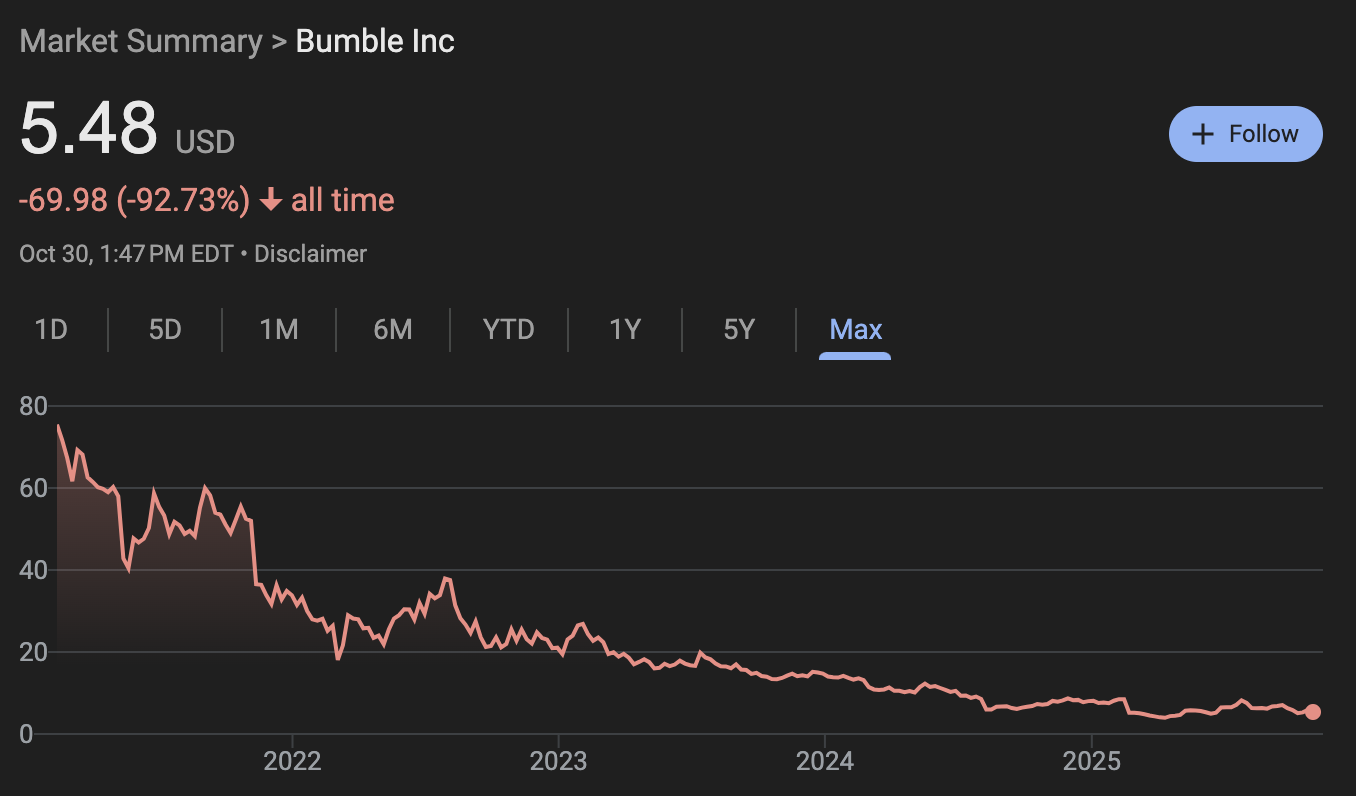
\includegraphics[height = .8\textheight]{bumble_2.png}
\end{center}
    
\end{frame}


\begin{frame}{Economics of Matching Markets}

\begin{itemize}
    \item As of 2023, 10\% of partnered Americans met their significant other on an app 
    \item Despite this, Bumble and Match Group (-63\%) IPOs have been disasters for equity investors \pause 
    \item If your matching algorithm is too good, users leave! 
    \begin{itemize}
        \item Fundamental conflict between product quality and revenue \pause 
    \end{itemize}
    \item Uber problem: why don't riders pay drivers in cash, off-app, to avoid paying the network's cut? \pause 
    \begin{itemize}
        \item App will ban a driver who cancels too many rides \pause
        \item Many dating app customers are (or hope to be) one-time players! Can't punish them with future exclusion from the marketplace. 
    \end{itemize}
    \item An opportunity for DeFi? 
\end{itemize}
    
\end{frame}



\begin{frame}{Trump CFPB Dismisses Moneygram Complaint}

\begin{center}
    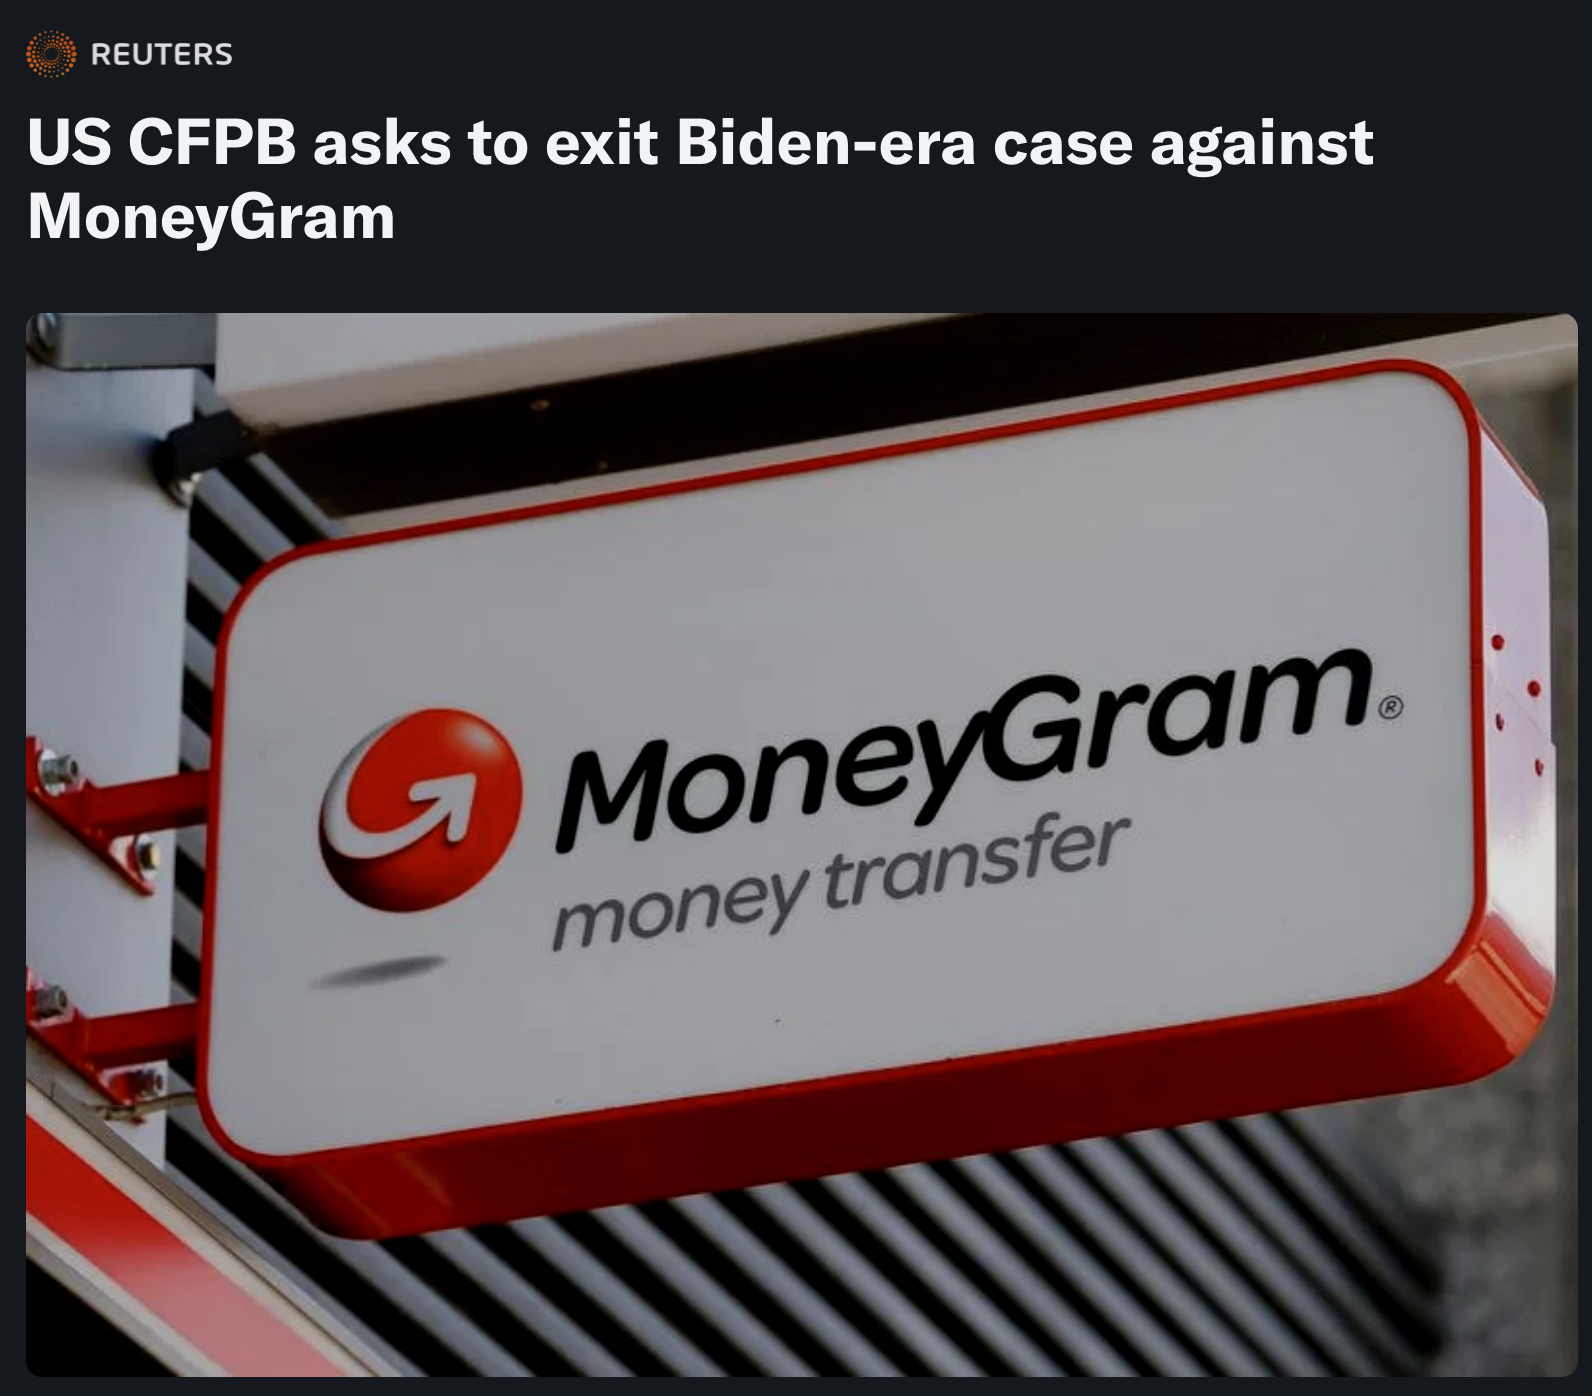
\includegraphics[height = .8\textheight]{Crowdfunding/moneygram_headline.png}
\end{center}
    
\end{frame}

\begin{frame}{Moneygram Business Model}

\begin{center}
    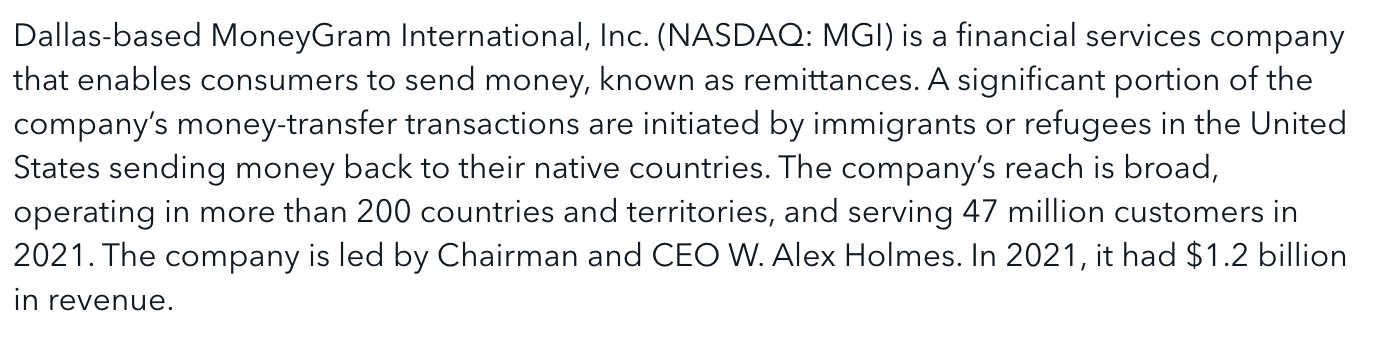
\includegraphics[width = \textwidth]{Crowdfunding/moneygram_description.png}
\end{center}
    
\end{frame}

\begin{frame}{Moneygram Complaint}

\begin{center}
    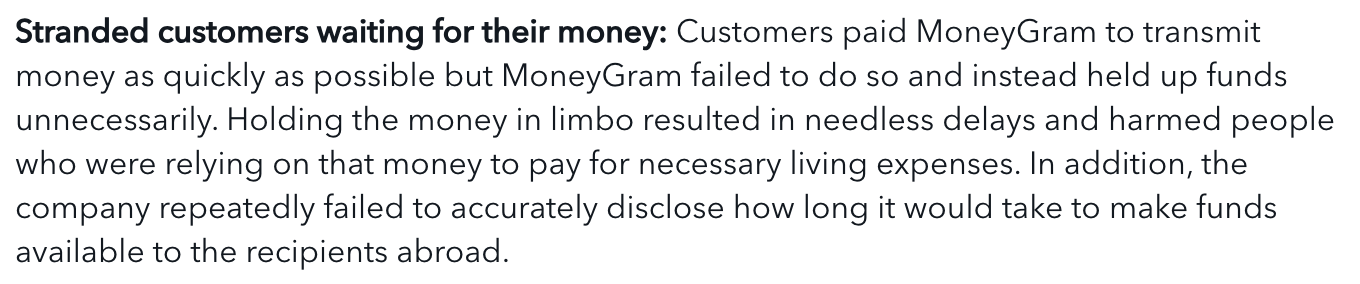
\includegraphics[width = \textwidth]{Crowdfunding/moneygram_complaint.png}
\end{center}
    
\end{frame}

\begin{frame}{Other Regulations Binding Moneygram}

\begin{center}
    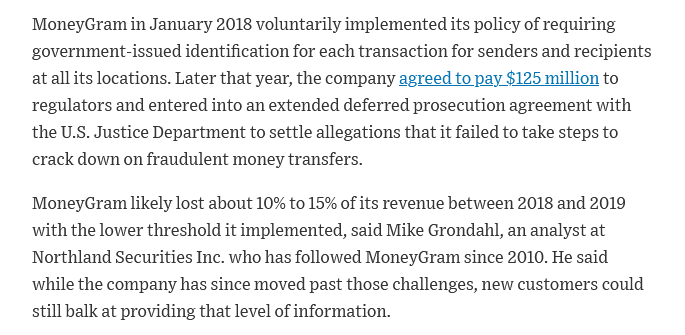
\includegraphics[width = \textwidth]{Crowdfunding/moneygram_AML.png}
\end{center}
    
\end{frame}

\begin{frame}{Circle Runs Circles Around Tether in On-Chain Velocity}

\begin{center}
    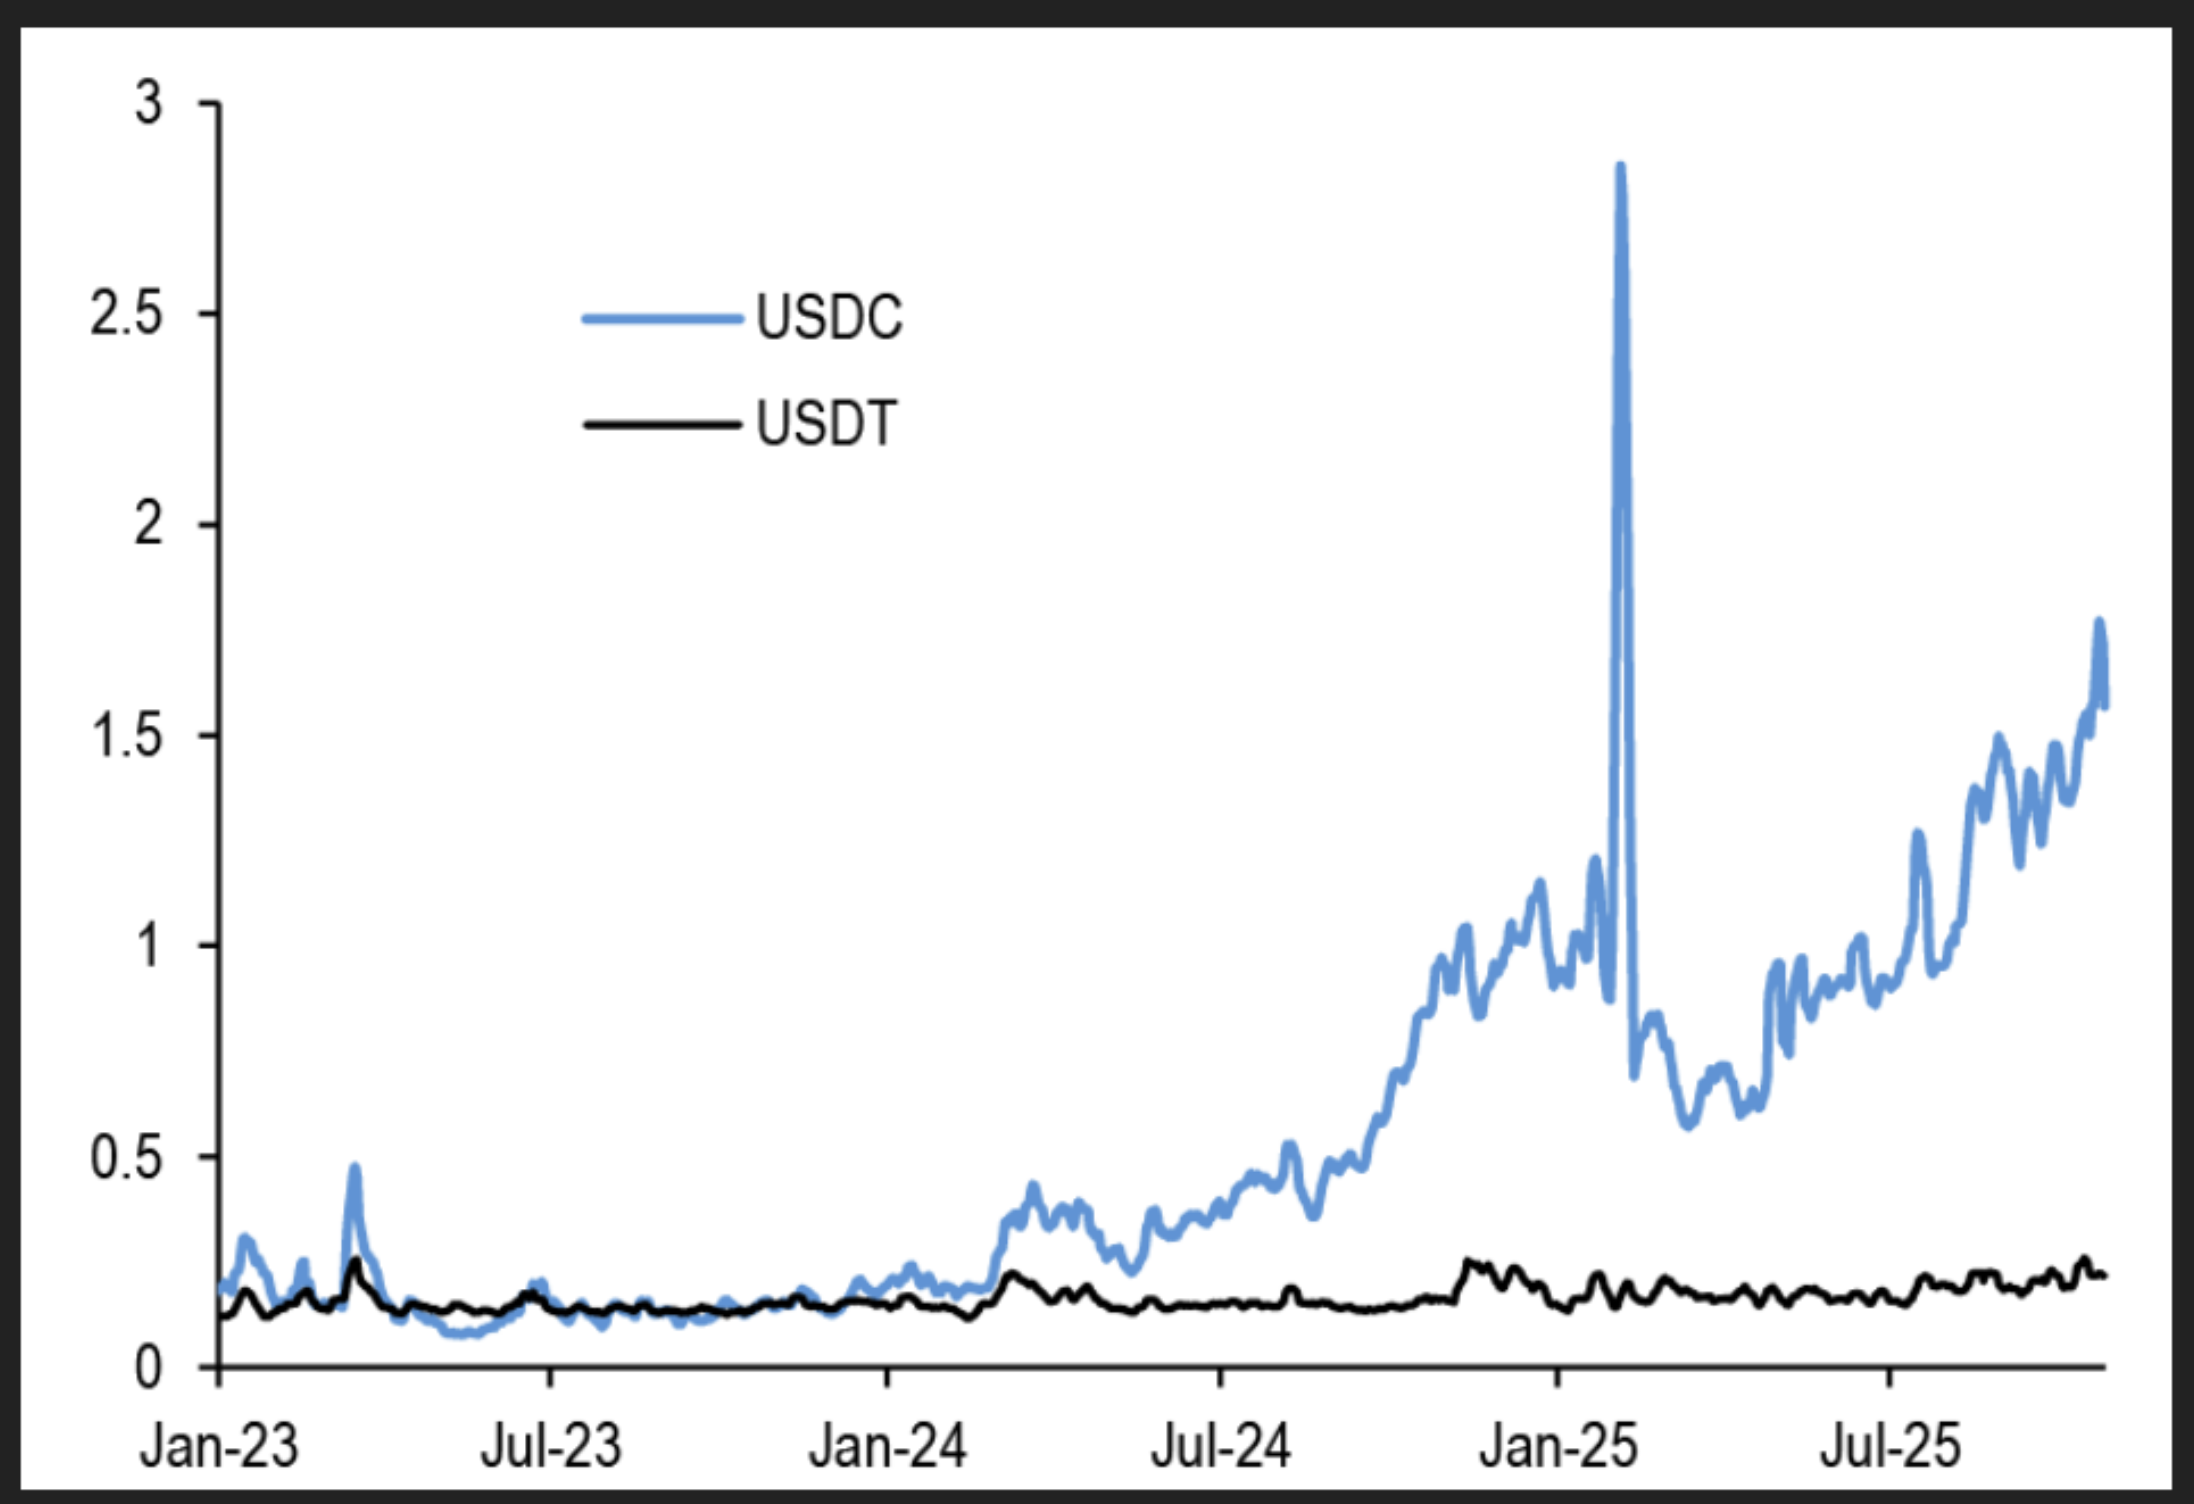
\includegraphics[height = .6\textheight]{circle_tether.png}
\end{center}

\bi
\m Tether still leads in market cap \href{https://www.coinbase.com/explore}{183B to 76B}
\m This chain velocity measure does not include L2s (why?) 
\ei 
Source: JP Morgan Flows \& Liquidity 
    
\end{frame}

\begin{frame}{Tether vs. Circle: Market Cap}

\begin{center}
    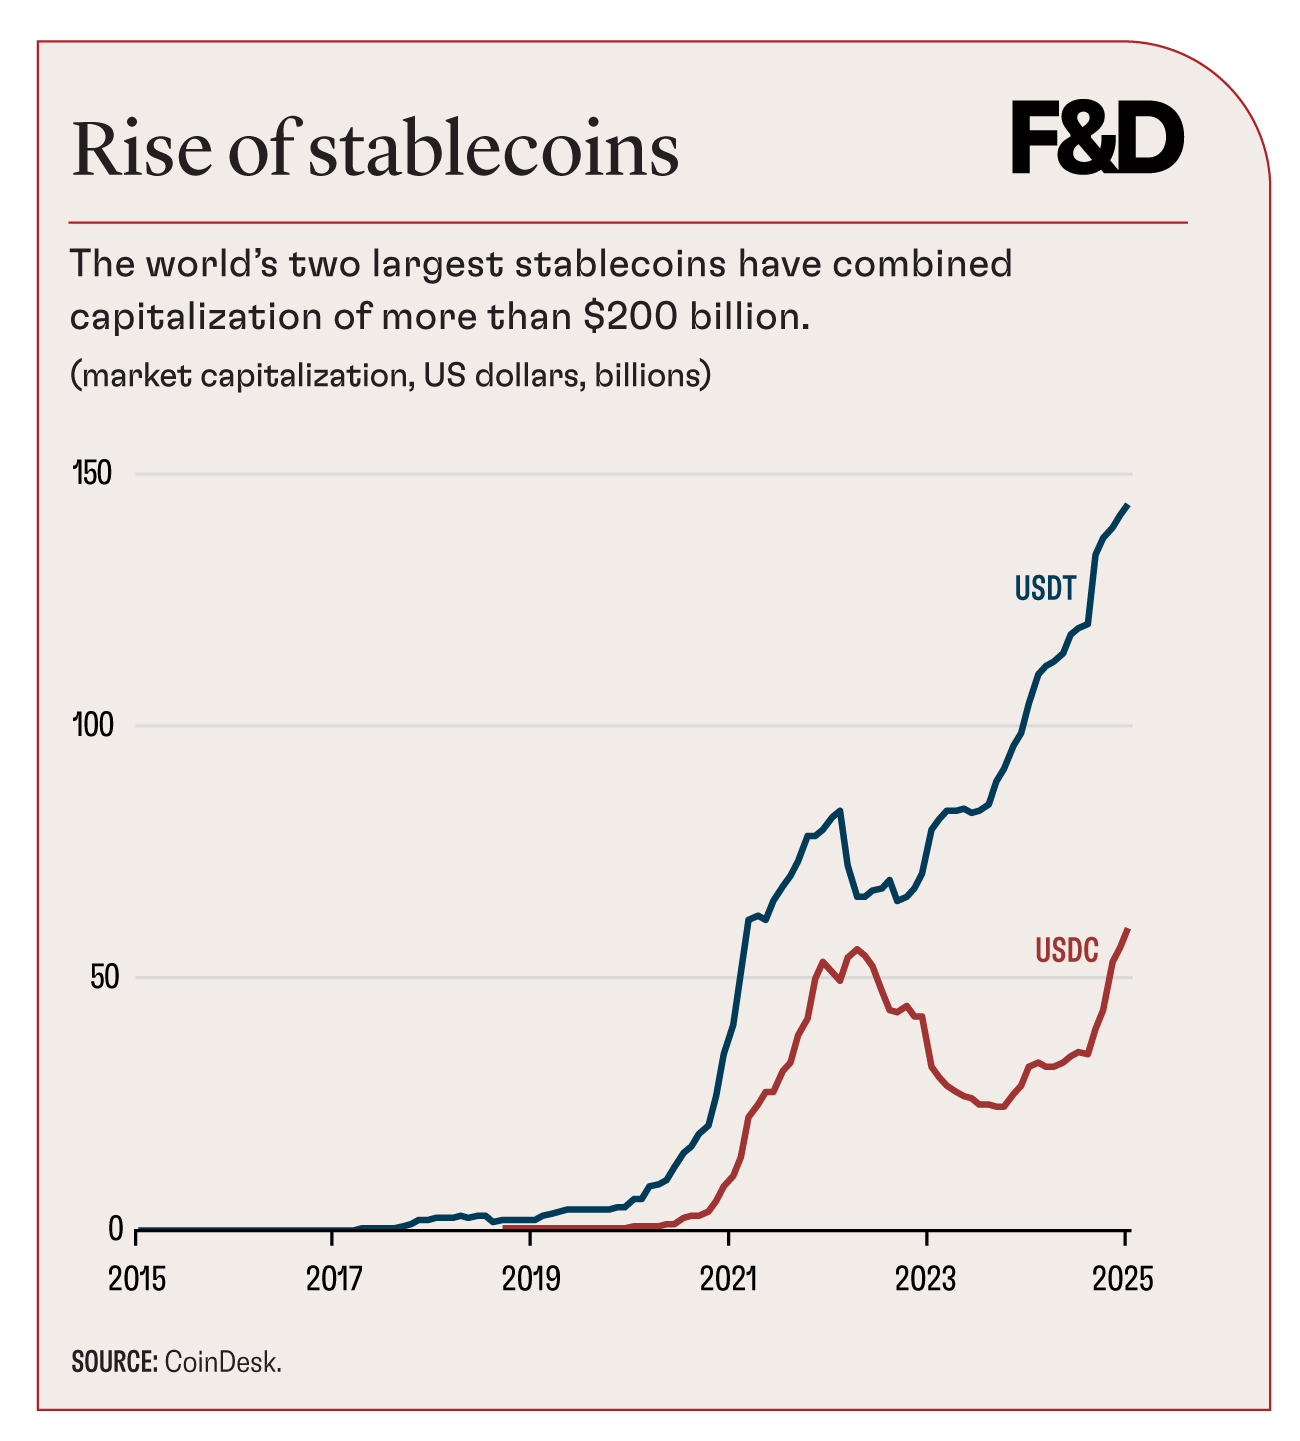
\includegraphics[height = .8\textheight]{stablecoin_marketcap.jpeg}
\end{center}
    
\end{frame}


\begin{frame}{Trump Pardons Binance Founder Changpeng Zhao}

CZ served four months and paid \$50 million fine, plus \$4.3 \emph{billion} paid by Binance, for ``Implementing a sham compliance program that would fool US regulators into believing they were screening for suspicious or illicit activity, while simultaneously allowing illicit transactions to continue unimpeded'' \\   

\vfill 

The indictment included hilarioius quotes unearthed by prosecutors, such as ``We are operating a fking unlicensed securities exchange in the USA bro'' from the Chief Compliance Officer. \\ \vfill

Source: \href{https://www.citationneeded.news/issue-95/}{Molly White for ``Citation Needed'' Newsletter}
    
\end{frame}


\section{Retail Fintech}

\begin{frame}{Summary}

\begin{itemize}
    \item ``Fintech'' in the context of lending is a loose term, generally referring to \textbf{non-bank lenders} who employ some kind of innovative business practice 
    \item Their innovation is usually in either \textbf{digital user experience}, \textbf{automated underwriting}, or both 
    \item They often rely on \textbf{bank partnership or licensing agreements} to do business, especially in the United States
    \item They live in \textbf{regulatory grey areas}, often relying on \textbf{prosecutorial discretion} to operate
    \item The simplest distinction is they \textbf{do not take deposits} and do not benefit from deposit insurance
    \item In finance, \textbf{retail} just means any high-volume business that accepts generic walk-in customers off the street 
\end{itemize}
    
\end{frame}
%----------------------------------------------------  


%------------------------------------------------

\begin{frame}
\frametitle{Retail Lending}


Retail Lending vs. Wholesale Lending \\

\begin{table}[H]
\centering
\begin{tabular}{@{}p{3.5cm}p{4.5cm}p{4.5cm}@{}}
\toprule
\textbf{Feature} & \textbf{Retail Lending} & \textbf{Wholesale Lending} \\ 
\midrule
Target Customers & Individuals and Small Business & Large Corporations and Institutions\\
\hline 
Loan Size & Small to Medium & Large \\
\hline 
Volume & High volume, low value & Low volume, high value \\
\hline 
Underwriting Process & Standardized, automated & Customized, manual \\
\hline 
Risk Profile & Diversified across many borrowers & Concentrated in fewer borrowers \\
\hline 
Examples & Mortgages, credit cards, personal loans & Corporate loans, syndicated loans, interbank lending \\ 
\bottomrule
\end{tabular}
\end{table}


	
\end{frame} 
%----------------------------------------------------  




%------------------------------------------------

\begin{frame}
\frametitle{Retail Lending Sector Facts}

\vspace{-2mm}
Types of lenders in the retail lending sector:
\vspace{-2mm}

\begin{table}[H]
\centering

\resizebox{0.97\textwidth}{!}{%

\begin{tabular}{@{}>{\bfseries}m{3cm} | m{4cm} | m{4cm} | m{4cm} | m{4cm}@{}}
\toprule
Feature & Banks & Nonbank Financial Institutions & Crowdfunding / P2P Platforms & Fintech Lenders \\
\midrule
License & Full banking license & Lending license, no deposit-taking & Platform model, sometimes regulatory exemption & Lending license or bank partnerships \\
\hline 
Funding Source & Deposits, capital markets & Capital markets, retained earnings & Retail and institutional investors & VC, bank partnerships, securitization \\
\hline 
Tech Foundation & Legacy systems + digital upgrades & Traditional, slow to digitize & Platform-native & Digital-first, app-native \\
\hline 
Underwriting Approach & Credit scores, income verification & Traditional credit checks & Peer or social info, light underwriting & AI, alternative data, behavioral analytics \\
\hline 
Channels & Branch + online & Branch + limited digital & Online-only & Fully digital, mobile-first \\
\hline 
Customer Target & Broad: retail + businesses & Mostly individual consumers & Individuals and small businesses & Targeted niches (e.g., BNPL, students) \\
\hline 
Regulation Intensity & High (banking regulators) & Moderate & Varies by jurisdiction & Lighter, evolving regulatory environment \\
\hline 
Speed and UX & Moderate to slow & Moderate & Fast, depends on investor match & Instant, seamless digital experience \\
\hline 
Innovation Pace & Low to moderate & Low & Moderate to high & High, rapid innovation cycles \\
\bottomrule
\end{tabular}
%
} % end of resize box

\end{table}


	
\end{frame} 
%----------------------------------------------------  


%------------------------------------------------

\begin{frame}
\frametitle{Retail Lending Sector Facts}

\vspace{-2mm}
Banks alone are huge in retail lending (\textbf{CAGR} = "Cumulative Annual Growth Rate"): 
\vspace{-4mm}
%-----------------------------------------------
\begin{figure}[H]
    \resizebox{5in}{2.1in}{%
    %\resizebox{\textwidth}{!}{%
    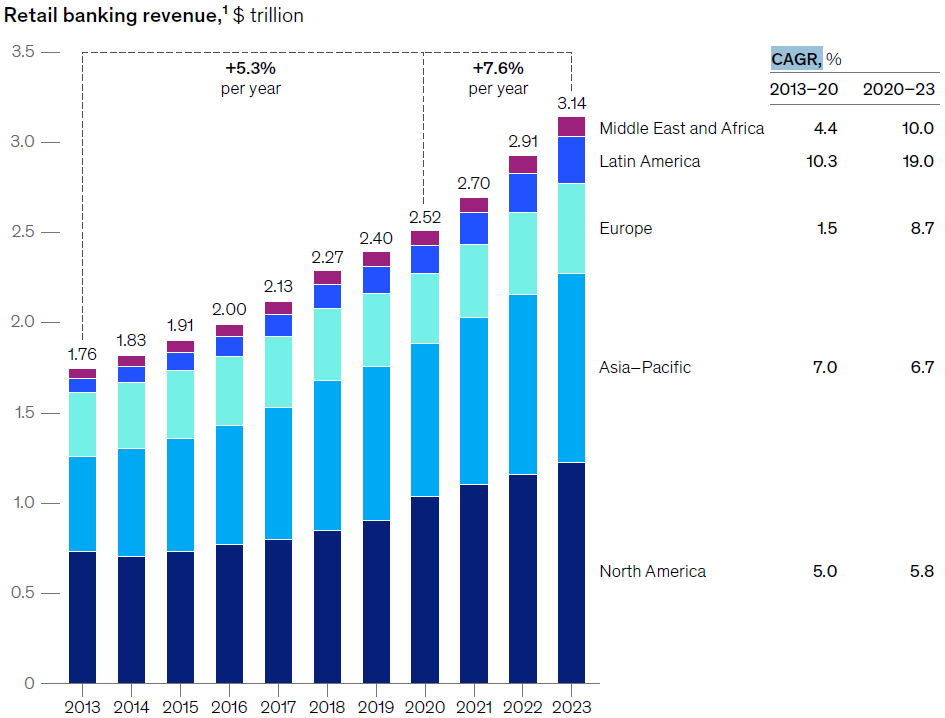
\includegraphics[]{Crowdfunding/figures/GlobalRetailLendingMarket_OnlyBank_ByArea.png}
    } %end of resizebox
%-----------------------------------------------
% Figure setting: caption and label
%-----------------------------------------------
%\caption{}
%\label{fig:ModelIntuition_Graphs}
\end{figure}
%-----------------------------------------------
\vspace{-3mm}








	
\end{frame} 
%----------------------------------------------------  




%------------------------------------------------

\begin{frame}
\frametitle{Retail Lending Sector Facts}



{\footnotesize Unlike regulated banks, public data is not reliable for Non-bank financial institutions, crowdfunding \& P2P platforms, and FinTech lenders!} 


\medskip 

However, Philipp Schnabl (NYU) and Manasa Gopal (Georgia Tech) study Uniform Commercial Code (``\textbf{UCC}'') filings of securitized, non-real-estate U.S. business loans made by non-banks (``fintechs'')

{\small 
\begin{itemize}
    \item Creditors have the right to file a record with the UCC registry specifying a loan and the underlying collateral, which is referred to as a ``UCC filing". 
    \item A UCC filing records the security interest in the underlying asset, analogous to mortgages for real estate, and determines the priority order of creditors in bankruptcy.
    \item If the borrower pledges a piece of collateral to multiple lenders, the lender with the earliest filing date has priority over other lenders.
\end{itemize}
 }


	
\end{frame} 
%----------------------------------------------------  




%------------------------------------------------

\begin{frame}
\frametitle{Retail Lending Sector Pain Points}




\vspace{-5mm}
%-----------------------------------------------
\begin{figure}[H]
    \resizebox{4.6in}{2in}{%
    %\resizebox{\textwidth}{!}{%
    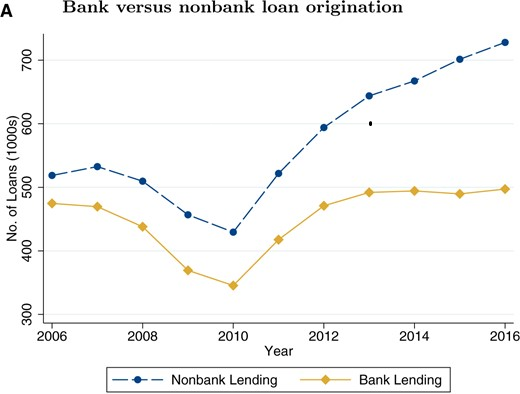
\includegraphics[]{Crowdfunding/figures/GrowthOfNonbankLending_Post2008.png}
    } %end of resizebox
%-----------------------------------------------
% Figure setting: caption and label
%-----------------------------------------------
%\caption{}
%\label{fig:ModelIntuition_Graphs}
\end{figure}
%-----------------------------------------------
\vspace{-3mm}
{\footnotesize Note: nonbank lending here includes all lending that are not by bank. }

\smallskip 
\vspace{1mm}


Schnabl \& Gopal (2022) find that heavier regulatory cost on banks post-2008 is one explanation for the relatively faster growth of nonbank lending.

\end{frame} 
%----------------------------------------------------  





%------------------------------------------------


%----------------------------------------------------  




\section{Passive Investing and ETFs}

%----------------------------------------------------  
%----------------------------------------------------  




%------------------------------------------------

\begin{frame}
\frametitle{Passive Investing and ETFs}


Passive investing has gained momentum over active investing, with ETFs increasingly replacing mutual funds.
    

\begin{itemize}
        \item Modern portfolio theory (Mainly the Capital Asset Pricing Model, or ``CAPM'') laid the groundwork for the growth of passive investing, also called index investing.
        \begin{itemize}
            \item Developed by Nobel Prize laureates Harry Markowitz, William Sharpe, and their peers.
             \item Passive investing does not rely on skill or technical analysis to beat the markets through security selection or timing.
        \item Instead, it focuses on tracking broad market indices and minimizing fees.
        \end{itemize}
       
    \item John Bogle, founder of Vanguard Group, created the first index mutual fund in 1975.
    \begin{itemize}
        \item Vanguard’s low-cost, passive mutual funds and ETFs now manage more than \$8 trillion across 422 funds.
    \end{itemize}
\end{itemize}



\end{frame} 
%----------------------------------------------------  


\begin{frame}{Capital Asset Pricing Model}

\begin{center}
    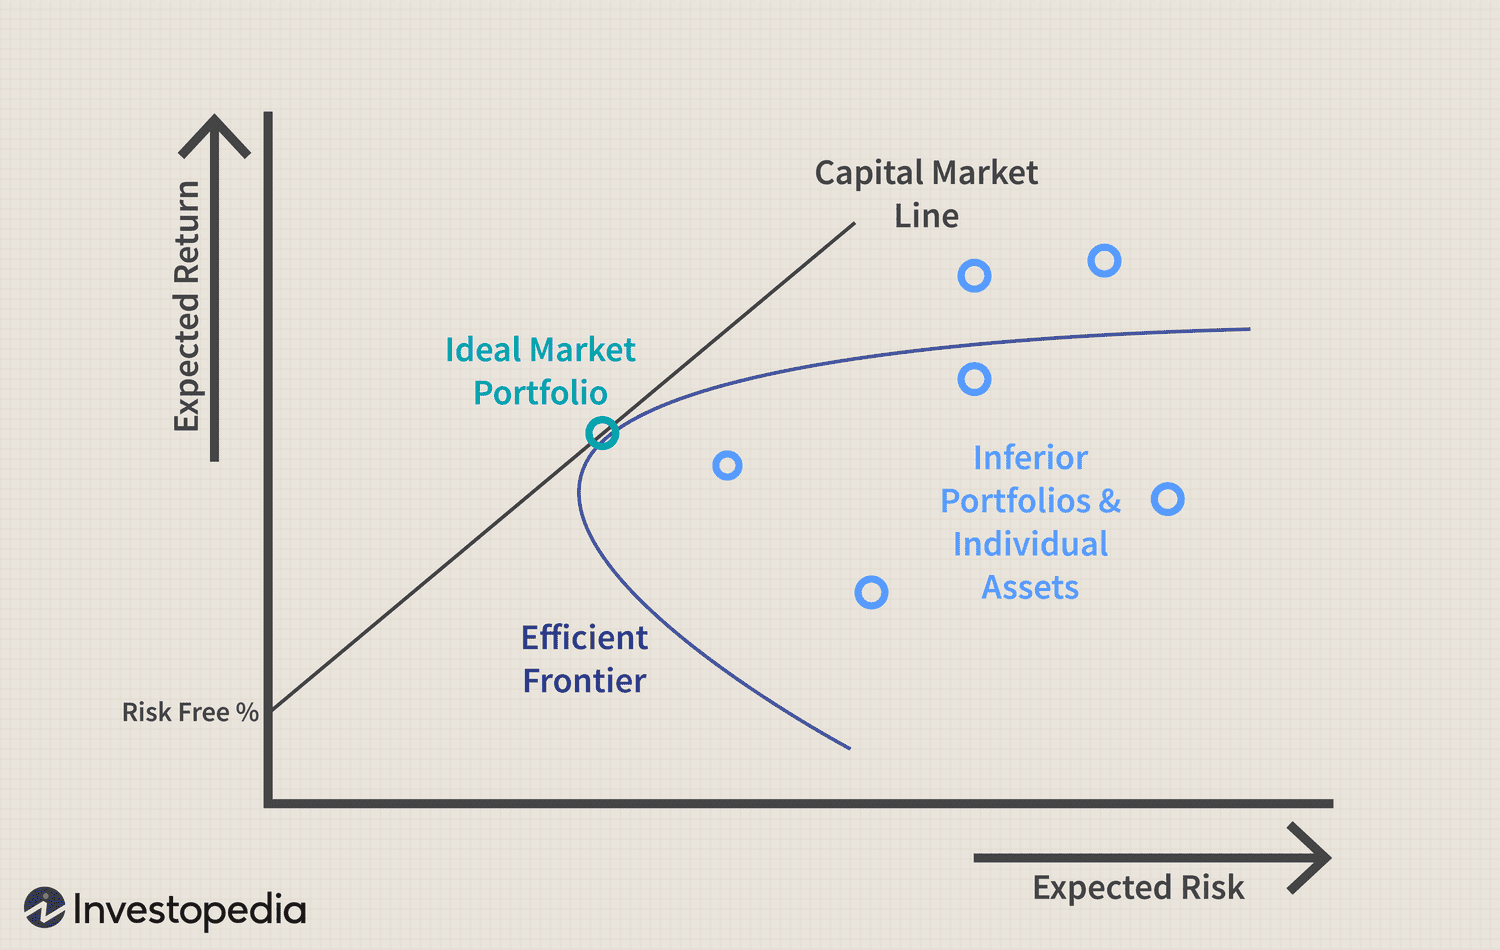
\includegraphics[height = .9\textheight]{capm.png}
\end{center}
    
\end{frame}

\begin{frame}{Capital Asset Pricing Model}

The CAPM is the workhorse model of modern financial advice.  

\begin{itemize}
    \item The CAPM assumes:
    \begin{enumerate}
        \item Markets are frictionless (no fees or minimum purchases)  
        \item Returns and covariances of all assets are common knowledge 
        \item All investors prefer high returns and low variance 
    \end{enumerate}
\end{itemize}

\textbf{If these assumptions hold}, it can be proven that: 
\begin{itemize}
    \item The total market index fund is the optimal asset
    \item There is no reason to pay an advisor any fee, as any investment they recommend is inferior to the total market index fund 
\end{itemize}



    
\end{frame}

\begin{frame}{Capital Asset Pricing Model}

 The CAPM formula says that the \textbf{only} differences in expected returns are explained by correlation with the market. 
 \vfill 
 In other words, the \textbf{only} way to get high returns is to add leverage (increase variance). 

$$E[r]= \beta\times E[r_m-r_f]+r_f$$

Where 

$$\beta = \frac{Cov(r,r_m)}{Var(r_m)}$$

\vfill 

If a portfolio manager claims to beat the market, be skeptical! Most so-called ``alpha'' is actually ``levered beta''. 

\end{frame}

\begin{frame}{It gets worse for financial advisors}

Even if the assumptions are wrong, and financial advisors can add value, \textbf{you}, the advisee, will not benefit from that value! Two reasons: \pause 
\begin{enumerate}
    \item Better managers will charge you higher \textbf{fees}
    \item Better managers will increase their fund size and move the price against them as they make larger and larger trades (``\textbf{price impact}'') 
\end{enumerate} \pause 

\vfill 
From \href{https://www.gsb.stanford.edu/faculty-research/research/publications/mutual-fund-flows-performance-rational-markets}{Berk and Green (2024)}: 

`` Fund flows rationally respond to past performance in the model even though performance is not persistent and \emph{investments with active managers do not outperform passive benchmarks on average.} \pause The lack of persistence in returns \emph{does not imply} that differential ability across managers is nonexistent or unrewarded or that gathering information about performance is socially wasteful.'' 
    
\end{frame}


\begin{frame}{Estimated Benefits to Customizing Retirement Savings}

\href{https://mitsloan.mit.edu/shared/ods/documents?PublicationDocumentID=10586}{Duarte, Fonseca, Goodman and Parker (2024)} train a cutting-edge neural network to optimally save for retirement in the presence of a wide variety of realistic frictions and quirks (labor income, social security, unemployment insurance, etc... over 100 parameters!) 

\vfill \pause 

They compare this optimal solution to a simple target-date fund (``TDF''). \\ 
\textbf{Question}: What \% of lifetime wealth does the optimal solution earn you, relative to the TDF? 

\vfill \pause 

\textbf{Answer}: 3\% (that does not compound -- that is the total). 

    
\end{frame}


%------------------------------------------------

\begin{frame}
\frametitle{Passive Investing and ETFs}

\vspace{-2mm}
Passive index funds have grown in popularity globally 

\vspace{-2mm}
\begin{itemize}
    \item Investors have focused on the high fees charged by asset managers and their underperformance relative to market benchmarks.
    

    \item Active managers charge a management expense ratio (MER) of 1\% to 2\% of AUM each year, as well as other fees (front-end and back-end load).
    
    \begin{itemize}
        \item A MER measures the fund’s annual operating expenses as a percentage of AUM. It includes management salaries, marketing and administration costs, and distribution costs.
    \end{itemize}

    \item Only 25\% of all active funds delivered a higher return than passive funds over the decade ending in 2021.

    \item The market share of actively managed funds has fallen from 81\% in 2010 to 60\% in 2020.
\end{itemize}



\end{frame} 
%----------------------------------------------------  



%------------------------------------------------

\begin{frame}
\frametitle{Passive Investing and ETFs}



\vspace{-2mm}
An Exchange Traded Fund (ETF) is an investment fund that trades on a stock exchange, like a share.

\begin{itemize}
    \item Each ETF holds a portfolio of securities such as stocks, bonds, or other asset classes.
    

    \item An ETF charges a MER between 0.03\% and 1.00\%, has no minimum investment, and trades throughout the day like a stock.

    \item ETFs were created as a cheaper, more liquid substitute to mutual funds.
    \begin{itemize}
        \item The first ETF, created in 1993, was the Standard \& Poor’s Depositary Receipts (SPDR), tracking the S\&P 500. It is the largest ETF in the world with \$450 billion AUM at year-end 2022.
        \item ETFs are available for different
        \begin{itemize}
            \item Asset classes: stocks, bonds, commodities, precious metals, bitcoin, real estate
            \item Sectors: health care, technology
            \item Markets and regions: emerging markets, Japan
            \item Strategies: currency hedged, low volatility, dividend income
        \end{itemize}
    \end{itemize}
\end{itemize}


\end{frame} 
%----------------------------------------------------  






%------------------------------------------------

\begin{frame}
\frametitle{Passive Investing and ETFs}

The value of ETFs passed \$10 trillion in 2023 with more than 10,250 ETFs traded globally.



\vspace{-2mm}
%-----------------------------------------------
\begin{figure}[H]
    \resizebox{5in}{2.4in}{%
    %\resizebox{\textwidth}{!}{%
    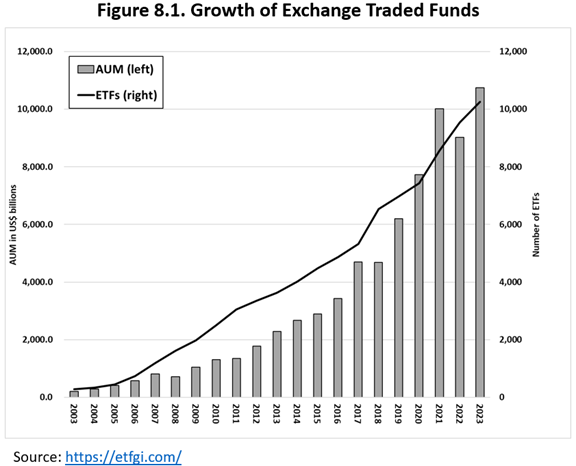
\includegraphics[]{figures/GrowthOfExchangeTradedFunds.png}
    } %end of resizebox
%-----------------------------------------------
% Figure setting: caption and label
%-----------------------------------------------
%\caption{xxxxxxxxxxxxxxxxxxxx}
%\label{fig:ModelIntuition_Graphs}
\end{figure}
%-----------------------------------------------
\vspace{-2mm}



\end{frame} 
%----------------------------------------------------  



%----------------------------------------------------  
%----------------------------------------------------  
%\section{How Robot Advisors Transformed the Wealth Management Sector}
%----------------------------------------------------  
%----------------------------------------------------  




%------------------------------------------------

\begin{frame}
\frametitle{Robinhood’s Commission-Free Trading}


\begin{itemize}
    \item In 2014, Robinhood launched a mobile trading app with the mission to democratize finance.
    \begin{itemize}
        \item Co-founders Vlad Tenev and Baiju Bhatt were Stanford roommates who worked in high-frequency trading.
        \item The app offered zero-commission trading for younger, less wealthy millennial investors.
        \item Claimed revenue would come from margin trading and securities lending.
        \item Raised \$3 million seed funding in 2013; approved by FINRA to operate as a broker-dealer.
    \end{itemize}
    \item Rapid growth: 2 million customers by 2017, 6 million by 2018, 10 million by 2019.
    \begin{itemize}
        \item In 2019, raised \$323 million in Series E funding; valued at \$7.6 billion.
    \end{itemize}
\end{itemize}


\end{frame} 
%----------------------------------------------------  



%------------------------------------------------

\begin{frame}
\frametitle{Robinhood’s Commission-Free Trading}


\vspace{-2mm}
\begin{itemize}
    \item 2019: FINRA fined Robinhood \$1.25M by FINRA for violations related to customer equity orders
    \begin{itemize}
        \item Directed trades to 4 broker-dealers who paid for order flow. Did not get much attention though…
    \end{itemize}
    \item 2020 COVID-19 hit;  online retail trading exploded
    \begin{itemize}
        \item \$280 million Series F funding, \$8.3 billion valuation
    \end{itemize}
    \item Aug 2020 Fortune ``The Inside Story ..."
\end{itemize}



\vspace{-6mm}
%-----------------------------------------------
\begin{figure}[H]
    \resizebox{5.6in}{1.3in}{%
    %\resizebox{\textwidth}{!}{%
    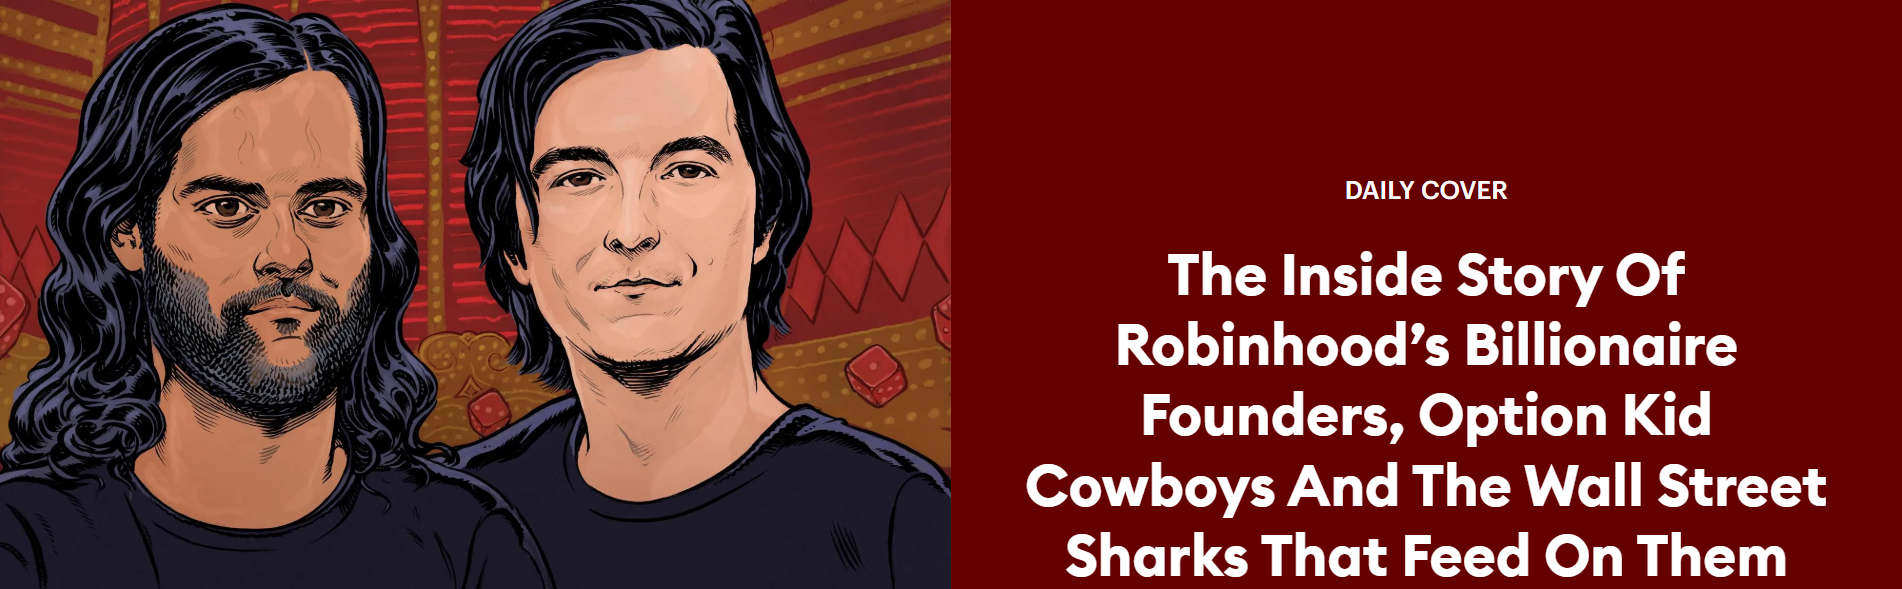
\includegraphics[]{figures/2020FortuneTitle.png}
    } %end of resizebox
%-----------------------------------------------
% Figure setting: caption and label
%-----------------------------------------------
%\caption{Insurtech Performance First Year Post-IPO}
%\label{fig:ModelIntuition_Graphs}
\end{figure}
%-----------------------------------------------
\vspace{-2mm}


\end{frame} 
%----------------------------------------------------  


%------------------------------------------------

\begin{frame}
\frametitle{Robinhood’s Commission-Free Trading}


\vspace{-2mm}
\begin{itemize}
    \item \textit{“The perfect stock trading app for the videogame generation was supposed to 'democratize finance' with zero-commission trades. But the primary plan was to get rich by selling customer trades to the market’s most notorious operators.”} — \textbf{Fortune, Aug 19, 2020}
    \item Story exposed Robinhood’s monetization strategy, called \textbf{payment for order flow}.
    \begin{itemize}
        \item Sophisticated proprietary traders pay Robinhood for the privilege of being the counterparties to unsophisticated retail traders 
        \item If you are getting a service for free, \emph{you are the product!}
    \end{itemize}
\end{itemize}


\end{frame} 
%----------------------------------------------------  


%------------------------------------------------

\begin{frame}
\frametitle{Robinhood’s Commission-Free Trading}




\vspace{-2mm}
\begin{itemize}
    \item Retail investors continued to flock to Robinhood, with customers hitting 12.5 million
    \begin{itemize}
        \item Aug 2020 \$200 million Series G, \$11.2 billion valuation
    \end{itemize}
    \item January 2021 Meme stock craze where retail squeezed shorts
    \begin{itemize}
        \item Sharp rise in GameStop stock led Robinhood to restrict trading for several days, infuriating retail traders.
        \item DTCC demanded Robinhood post \$3 billion in cash as collateral against risky trades by its customers;
        \item Raised over weekend from existing investors
        \item Feb and Mar 2020: Ordered to give testimony to Congress
    \end{itemize}
    \item July 2021 Robinhood priced IPO at \$38 per share, or \$31.7 billion valuation
    \begin{itemize}
        \item Co-founders worth \$5 billion
    \end{itemize}
\end{itemize}


\end{frame} 
%----------------------------------------------------  



%------------------------------------------------

\begin{frame}
\frametitle{Robinhood’s Commission-Free Trading}

%\vspace{-2mm}
%Robinhood stock fell by -78\% to \$7.70 at end 2022

%-----------------------------------------------
%\begin{figure}[H]
%    \resizebox{4.6in}{2in}{%
    %\resizebox{\textwidth}{!}{%
    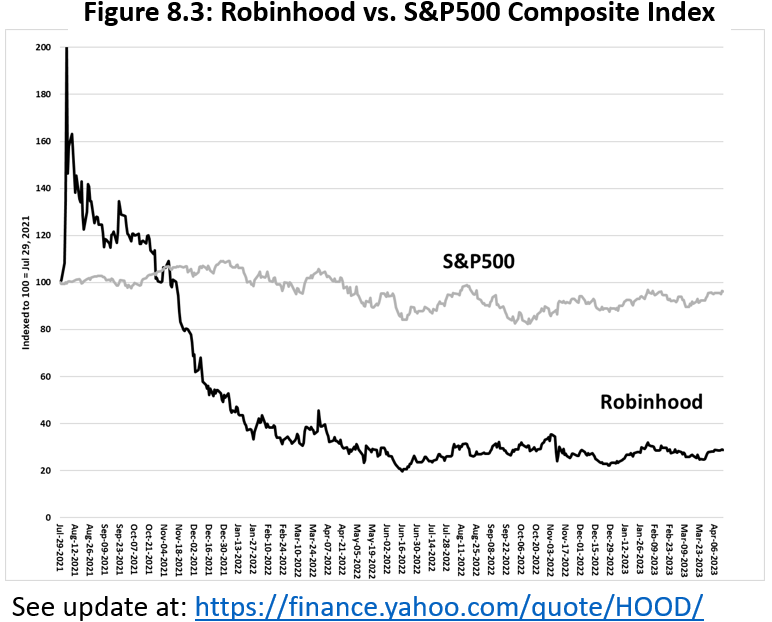
\includegraphics[height = .8\textwidth]{figures/Robinhood_StockPrice.png}
%    } %end of resizebox
%-----------------------------------------------
% Figure setting: caption and label
%-----------------------------------------------
%\caption{Insurtech Performance First Year Post-IPO}
%\label{fig:ModelIntuition_Graphs}
%\end{figure}
%-----------------------------------------------
%\vspace{-2mm}


\end{frame} 
%---------------------------------------------------- 






%---------------------------------------------------- 
\section{Robot Advisors}
%---------------------------------------------------- 


%------------------------------------------------

\begin{frame}
\frametitle{Robot Advisors Basics}

\vspace{-2mm}

Robo-Advisors: Spoiler Alert – Goliath Beats David

\smallskip 
\begin{itemize}
  \item Robo-advisors offer automated online investment using algorithms to provide personalized portfolio recommendations.
  \item Emerged in 2008 as low-cost, simple alternatives for DIY investors or those avoiding financial advisors.
  \item Despite early attention, most independent robo-advisors were either shut down or acquired.
  \item As of 2022, robo-advisors manage \$1.8 trillion — less than 2\% of the \$100 trillion global wealth management market.
  \item The gap between ``too poor for your asset allocation to really matter'', and ``rich enough to hire a real person'' might just not exist. 
  
%  \smallskip 
%  \item \textbf{Insight:} Robo advice has succeeded through adoption by major financial institutions, not disruption by startups.
\end{itemize}



\end{frame} 
%----------------------------------------------------  



%------------------------------------------------

\begin{frame}
\frametitle{Robot Advisors Basics}


\vspace{-2mm}
The Rise of the Robo-advisor
\begin{itemize}
  \item Robos automate investment for retail customers and charge a low fee, 0.25\% to 0.50\% of assets under management (AUM).
  \begin{itemize}
      \item Most human wealth advisors charge 1-3\% 
  \end{itemize}

  \item You connect over the internet or a mobile app, then answer questions about: (1) your savings goals; (2) return expectations; (3) risk tolerance

  \item The robo algorithm maps your answers to a portfolio recommendation that is implemented automatically once funds are transferred into an account.

  \item Money is invested in low-cost exchange traded funds (ETFs), typically a 60/40 mix of equities and bonds.

  \item The portfolio is automatically rebalanced: quarterly, monthly, or daily, to maintain the target asset allocation.
  

  \item It is all shown on a simple, clean \& attractive dashboard.

\end{itemize}



\end{frame} 
%----------------------------------------------------  



%------------------------------------------------

\begin{frame}
\frametitle{Robot Advisors and the Wealth Management Sector}


\vspace{-2mm}
The Early Disruptors
\begin{itemize}
    \item The first U.S. robo-advisor, \textbf{Betterment}, was founded in 2007 and launched in 2010.
    \begin{itemize}
        \item Followed by: Wealthfront (2011); Personal Capital (2011); FutureAdvisor (2012) 
        \item Robo-advisors also appeared globally: \textbf{Canada:} Nest Wealth, Wealthsimple; \textbf{UK:} Nutmeg; \textbf{Australia:} Stockspot, Raiz; \textbf{Europe:} MoneyFarm, OwlHub
    \end{itemize}
\end{itemize}



\vspace{-5mm}
%-----------------------------------------------
\begin{figure}[H]
    \resizebox{5.6in}{1.8in}{%
    %\resizebox{\textwidth}{!}{%
    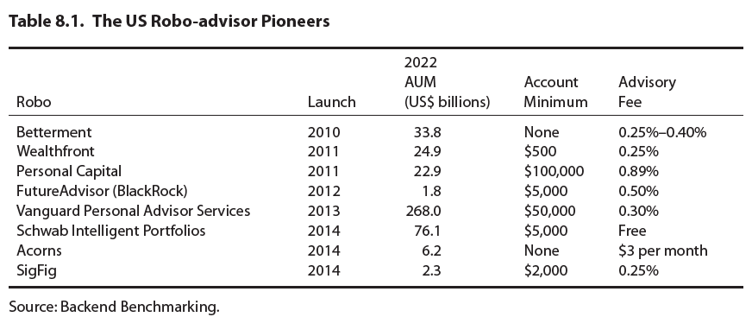
\includegraphics[]{figures/USRobotAdvisorPioneers.png}
    } %end of resizebox
%-----------------------------------------------
% Figure setting: caption and label
%-----------------------------------------------
%\caption{xxxxxxxxxxxxxxxxxxxx}
%\label{fig:ModelIntuition_Graphs}
\end{figure}
%-----------------------------------------------
\vspace{-2mm}




\end{frame} 
%----------------------------------------------------  




%------------------------------------------------

\begin{frame}
\frametitle{BlackRock’s Aladdin Platform}



\vspace{-2mm}
\begin{itemize}
    \item BlackRock has been licensing its in-house portfolio management platform, Aladdin, to institutional investors, corporations, and financial advisors.
    \begin{itemize}
        \item Aladdin stands for Asset Liability, Debt and Derivative Investment Network.
        \item  It is licensed to 16 retail wealth management firms including JPMorgan Stanley and UBS Group.
    \end{itemize}
    \item The platform combines front, middle, and back-office functions for managing client portfolios.
    \begin{itemize}
        \item It helps build portfolios aligned with investors’ goals and risk tolerance.
        \item Advisors can show clients their investments, exposure to risk, and performance.
    \end{itemize}
\end{itemize}



\vspace{-6mm}
%-----------------------------------------------
\begin{figure}[H]
    \resizebox{5.6in}{1in}{%
    %\resizebox{\textwidth}{!}{%
    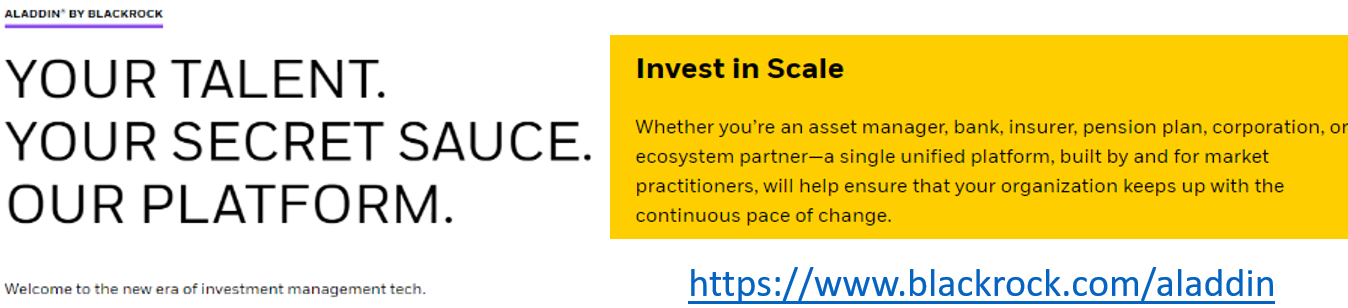
\includegraphics[]{figures/Blackrock_Aladdin.png}
    } %end of resizebox
%-----------------------------------------------
% Figure setting: caption and label
%-----------------------------------------------
%\caption{Insurtech Performance First Year Post-IPO}
%\label{fig:ModelIntuition_Graphs}
\end{figure}
%-----------------------------------------------
\vspace{-2mm}





\end{frame} 
%----------------------------------------------------  






%------------------------------------------------

\begin{frame}
\frametitle{Robot Advisors and the Wealth Management Sector}


\vspace{-2mm}
Robot Advisors have gained a foothold in two customer segments:
\medskip 

\begin{itemize}
    \item Underserved customers: Millennials, especially HENRYs (High Earners, Not Rich Yet) with high expected lifetime wealth but no liquidity 
    \begin{itemize}
        \item Distrustful of incumbents
        \item Tech-savvy; preferred digital interface available 24/7
        \item Attracted to automated service, low minimum investments, and transparent fees
    \end{itemize}
    \medskip 
    \item \textbf{Price-sensitive customers}: Older individuals with \$100,000–\$1,000,000 to invest, unwilling to pay high advisory fees
    \begin{itemize}
        \item Did not want ancillary services bundled with advice
        \item DIY investors—by necessity, not by choice
        \item Wanted access to professional investment advice
    \end{itemize}
\end{itemize}



\end{frame} 
%----------------------------------------------------  



%------------------------------------------------

\begin{frame}
\frametitle{Robot Advisors and the Wealth Management Sector}


\vspace{-2mm}
The Robo-advisor Value Proposition is:  
\begin{itemize}
    \item \textbf{Customer experience}: fast, easy to use, enjoyable, and convenient (available 24/7)
    \smallskip 

    \item \textbf{Transparent, low fees}: Low or no minimum investment Advisory fee as low as 0.25\% of AUM or \$2/month
    \begin{itemize}
        \item Customers also pay MER of third-party ETFs (0.12\%–0.23\% of AUM)
    \end{itemize}
    \smallskip 

    \item \textbf{State-of-the-art technology}: not encumbered by the legacy computer systems of incumbents
    \smallskip 
    
    \item \textbf{Return-enhancing strategies}: annual, quarterly or daily tax-loss harvesting, multi-factor smart beta portfolios, risk parity portfolios. 

    \smallskip 

    \item \textbf{Speak to adviser}: many offer ability to speak to a financial advisor by phone or online chat
    
\end{itemize}




\end{frame} 
%----------------------------------------------------  


%------------------------------------------------

\begin{frame}
\frametitle{Lessons from Aspiring Disruptors}


\vspace{-2mm}
\begin{itemize}
    \item Main obstacle is \textbf{cost to acquire customers} (estimated at \$500+ in advertising and marketing).
    \begin{itemize}
        \item Average robo fee 0.35\% × \$10,000 account = \$35/year
        \item Payback period = \$500 / \$35 = 14.4 years
    \end{itemize}

    \item Technology is not a source of sustainable competitive advantage
    \begin{itemize}
        \item Widely available and can be copied by fast followers.
    \end{itemize}

    \item Consider \textbf{working with incumbents} (B2B), instead of attacking them (B2C)
    \begin{itemize}
        \item Pivoting to a B2B model and partnering with an incumbent is an attractive growth opportunity.
        
        \item Examples: Betterment for Advisors, SigFig, Wealthsimple for Advisors
        
    \end{itemize}
\end{itemize}


\end{frame} 
%----------------------------------------------------  




%---------------------------------------------------- 
%----------------------------------------------------
%\section{Case: Vanguard}
%---------------------------------------------------- 
%---------------------------------------------------- 


%------------------------------------------------

\begin{frame}
\frametitle{Vanguard’s Move into Robo-advice}


\vspace{-2mm}
In mid-2013 Vanguard began piloting in-house robo called \textit{Personal Advisor Services}.
\begin{itemize}
    \item Launched 2015 with a minimum account size of \$50,000
    \begin{itemize}
        \item Annual fee of 0.30\% for the first \$5 million in AUM, with rates declining for higher account balances.
        \item Recommended portfolio of low-fee Vanguard ETFs
    \end{itemize}
    \item By end 2018, \$112 billion, 50\% of U.S. robo industry
    \item By end 2022, \$268 billion: 3.5× AUM of Charles Schwab, and 4.6× combined AUM of Wealthfront + Betterment
\end{itemize}


\vspace{-5mm}
%-----------------------------------------------
\begin{figure}[H]
    \resizebox{5.6in}{1.2in}{%
    %\resizebox{\textwidth}{!}{%
    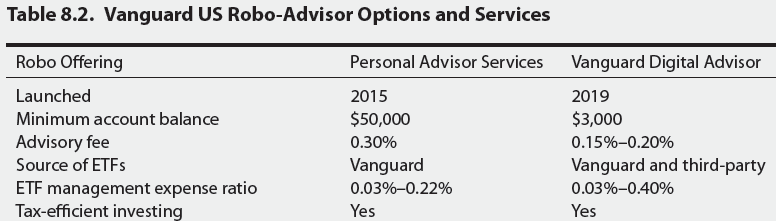
\includegraphics[]{figures/VanguardUSRoboAdvisorOptionsAndServices.png}
    } %end of resizebox
%-----------------------------------------------
% Figure setting: caption and label
%-----------------------------------------------
%\caption{xxxxxxxxxxxxxxxxxxxx}
%\label{fig:ModelIntuition_Graphs}
\end{figure}
%-----------------------------------------------
\vspace{-2mm}


\end{frame} 
%----------------------------------------------------  



%------------------------------------------------

\begin{frame}
\frametitle{Vanguard’s Move into Robo-advice}


\vspace{-2mm}
\href{https://investor.vanguard.com/advice/personal-hybrid-robo-advisor}{Website: Vanguard's personal-hybrid robo-advisor}

\vspace{1mm}

%------------------------------------
\begin{columns}
    \centering  
    \begin{column}{0.49\textwidth}
        \centering
        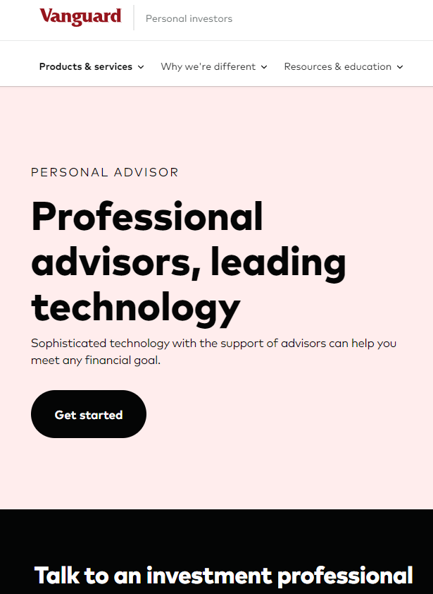
\includegraphics[width=2.8in, height=2.6in]{figures/VanguardRoboAdvisor_PageUp.png}
    \end{column}
    \hspace{0.4in}
    \begin{column}{0.49\textwidth}
        \centering 
        
\includegraphics[width=2.8in, height=2.6in]{figures/VanguardRoboAdvisor_PageDown.png}
    \end{column}
\end{columns} 
%------------------------------------
\vspace{-2mm}


\end{frame} 
%----------------------------------------------------  



%---------------------------------------------------- 
%----------------------------------------------------
%\section{Case: Wealthfront}
%---------------------------------------------------- 
%---------------------------------------------------- 


%------------------------------------------------

\begin{frame}
\frametitle{Wealthfront's Low-cost Sophisticated Robo-Advisor}


\vspace{-2mm}
Wealthfront provides \textbf{sophisticated financial advice to everyone at a low cost}

\begin{itemize}
        \item Co-founders: VC Andrew Rachleff, ex-trader Dan Carroll
        \item Rachleff saw portfolio modeling could be automated; left VC in 2005; teaching disruption to Stanford MBAs
        \item Tried different ideas over 3 years (e.g., crowd-based social investing on Facebook, mimic trades of professional investors)
\end{itemize}

\smallskip 

Pivoted to robo-advisor model in 2011
\begin{itemize}
    \item Hired 3 software engineers; built platform in 3 months
    \item Targeted millennials working at successful tech start-ups like Facebook and LinkedIn
    \item Customers complete questionnaire; maps to one of 20 risk profiles with associated asset allocation using ETFs 
\end{itemize}



\end{frame} 
%----------------------------------------------------  


%------------------------------------------------

\begin{frame}
\frametitle{Wealthfront's Low-cost Sophisticated Robo-Advisor}


\vspace{-2mm}
\begin{itemize}
    \item Grew through word-of-mouth.
    \begin{itemize}
        \item One-third of new clients acquired through referrals
        \item Spent \$0 on marketing, focused on product R\&D
        \item No human contact at all
        \item Charge low fees and still generate gross margin of 90\%
    \end{itemize}
    \medskip 
    
    \item Expanded services only if could be fully automated
    \begin{itemize}
        \item Tax-loss harvesting, multi-factor smart beta, risk parity strategies
        \item Customer insights and investment recommendations
        \item Diversified into financial planning including: Retirement, college, real estate, and time-off-to-travel planning
    \end{itemize}
    \medskip 
    
    \item In 2022 UBS offered to buy Wealthfront for \$1.4b
    \begin{itemize}
        \item Fell apart in late 2022 when UBS shareholders protested
    \end{itemize}
\end{itemize}


\end{frame} 
%----------------------------------------------------  


%------------------------------------------------

\begin{frame}
\frametitle{Wealthfront's Low-cost Sophisticated Robo-Advisor}


\vspace{-5mm}
%-----------------------------------------------
\begin{figure}[H]
    \resizebox{5.6in}{2.7in}{%
    %\resizebox{\textwidth}{!}{%
    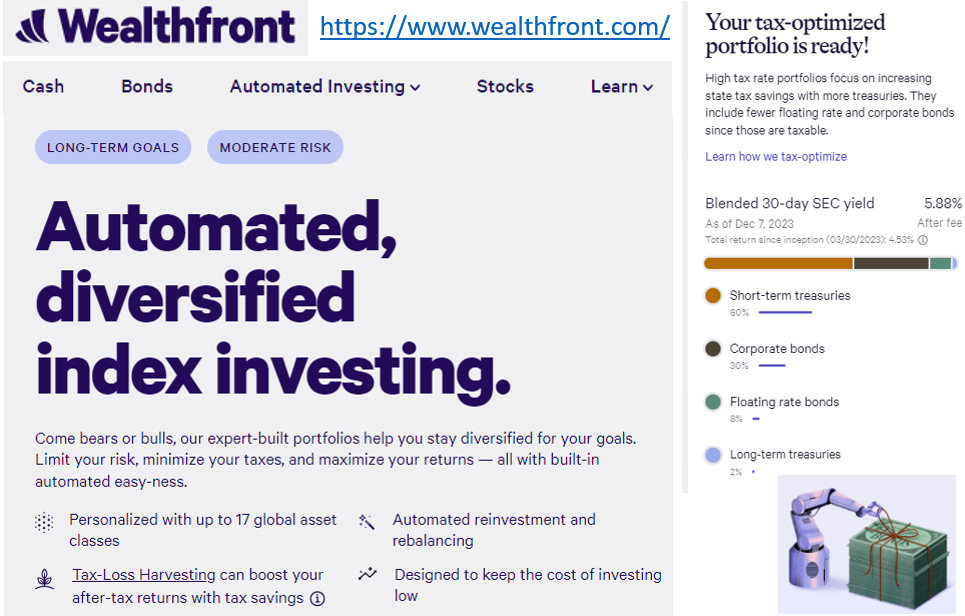
\includegraphics[]{figures/Wealthfront_Website.png}
    } %end of resizebox
%-----------------------------------------------
% Figure setting: caption and label
%-----------------------------------------------
%\caption{Insurtech Performance First Year Post-IPO}
%\label{fig:ModelIntuition_Graphs}
\end{figure}
%-----------------------------------------------
\vspace{-2mm}




\end{frame} 
%----------------------------------------------------  



%------------------------------------------------

\begin{frame}
\frametitle{Specialized Robot Advisors: ESG Investing}


\vspace{-2mm}
Sustainable Investing to Tackle Climate Change
\begin{itemize}
    \item In 2020, global sustainable investments reached \$35.3 trillion, or more than one-third of total AUM.
    \item Sustainable investing integrates environmental, social, and governance (ESG) factors into asset selection and portfolio construction. Also called responsible investing.
    \item Fintechs like UK's \textit{Clim8 Invest} provided a simple way to invest in clean energy, clean technology, sustainable food, clean water, and recycling.
    \begin{itemize}
        \item Clim8 offered two investment funds holding stocks, bonds, and ETFs.
        \item Customers could invest with as little as £25, choosing from three risk profiles: Cautious, Balanced, and Adventurous.
        \item Management fee was 0.60\% of AUM.
        \item Clim8 shut down in May 2023: growth was too slow and funding dried up
    \end{itemize}
\end{itemize}


\end{frame} 
%----------------------------------------------------  


%----------------------------------------------------  
%----------------------------------------------------  

%----------------------------------------------------  
%----------------------------------------------------  



%----------------------------------------------------  
%----------------------------------------------------  
%\section{The Wealth Management Industry}
%----------------------------------------------------  
%----------------------------------------------------  




%----------------------------------------------------  
%----------------------------------------------------  



%---------------------------------------------------- 
%---------------------------------------------------- 
\section{Crowdfunding}
%---------------------------------------------------- 
%---------------------------------------------------- 




%---------------------------------------------------- 
%---------------------------------------------------- 




%------------------------------------------------

\begin{frame}
\frametitle{Crowdfunding Basics}

\begin{itemize}
    \item Crowdfunding platforms allow individuals, businesses, and social causes to raise capital directly from the crowd in the form of debt, equity, donations, or rewards
    \begin{itemize}
        \item Also called alternative finance
        \item Debt crowdfunding platforms are Commonly called peer-to-peer (P2P) lenders or marketplace lenders
    \end{itemize}

    \medskip 

    \item These fintechs started between 2005 to 2009
    \begin{itemize}
        \item Zopa (UK), launched in 2005, was the pioneer among online portals
        \item OnDeck and Prosper launched in 2006; 
        \item CreditKarma and LendingClub in 2007; 
        \item Indiegogo and GoFundMe in 2008
        \item Funding Circle, Kabbage, and Kickstarter in 2009
    \end{itemize}

    \medskip 
    
    \item Described as the ``most disruptive way to raise money''
\end{itemize}


\end{frame} 
%----------------------------------------------------  






%------------------------------------------------

\begin{frame}
\frametitle{Crowdfunding Basics}

\begin{itemize}
    \item Technology made crowdfunding possible
    \begin{itemize}
        \item Fintechs leveraged the internet, mobile phones, software, APIs, cloud computing, and social media
    \end{itemize}
    \medskip 
    \item Platform growth
    \begin{itemize}
        \item In 2022, Crunchbase reported 1,500 active crowdfunding platforms headquartered in the USA
        \item An additional 200 platforms had closed
    \end{itemize}
    \medskip 
    \item Evolution of funding sources
    \begin{itemize}
        \item Originally crowdfunding was P2P, connecting individuals with retail investors ("the crowd")
        \item Now, most funding comes from institutional investors:
        \begin{itemize}
            \item Hedge funds, pension funds, insurance companies, banks, and professional investors
        \end{itemize}
        \item To reflect this broader capital source, the term \textbf{marketplace lending} is used
    \end{itemize}
\end{itemize}


\end{frame} 
%----------------------------------------------------  





%------------------------------------------------

\begin{frame}
\frametitle{Crowdfunding Basics}

\vspace{-2mm}
Business Models
\begin{itemize}
    \item Many crowdfunding platforms are multi-sided markets with users on various sides
\end{itemize}

\item Network effects are crucial: a higher number of users increases the value to:
\begin{itemize}
    \item The platform operator; The entity raising capital; The crowd(funders)
\end{itemize}


\vspace{-3mm}
%-----------------------------------------------
\begin{figure}[H]
    \resizebox{4in}{1.8in}{%
    %\resizebox{\textwidth}{!}{%
    
\includegraphics[]{Crowdfunding/figures/NetworkEffect.png}
    } %end of resizebox
%-----------------------------------------------
% Figure setting: caption and label
%-----------------------------------------------
%\caption{xxxxxxxxxxxxxxxxxxxx}
%\label{fig:ModelIntuition_Graphs}
\end{figure}
%-----------------------------------------------
\vspace{-3mm}




\end{frame} 
%----------------------------------------------------  










%------------------------------------------------

\begin{frame}
\frametitle{Crowdfunding Basics}

As crowdfunding finance has matured, \textcolor{red}{the hope} that online portals would disrupt banks and transform capital raising \textcolor{red}{has faded}.
\medskip 
\begin{itemize}
    \item Challenges faced by online portals
    \begin{itemize}
        \item Struggled to monetize users and cover the high customer acquisition costs: estimated at \$500 to \$1,000 per customer
        \item Disclosures of the largest, publicly listed online portals show years of losses with share prices falling steadily.
    \end{itemize}
    \medskip 
    \item Many platforms have pivoted from their original vision
    \begin{itemize}
        \item Closed to retail investors: Zopa, Prosper
        \item Became digital banks: LendingClub, SoFi
        \item Acquired by incumbents: Kabbage, OnDeck
        \item Many went bankrupt and disappeared
    \end{itemize}
\end{itemize}



\end{frame} 
%----------------------------------------------------  






%------------------------------------------------

\begin{frame}
\frametitle{Crowdfunding Basics}


Regarding the five dimensions of financial intermediation, Crowdfunding portals have succeeded in some areas but failed in others:

\begin{itemize}
    \item Reduced information asymmetry between savers and borrowers/investors by increasing disclosure


    \item Mixed on transaction costs; lowered the cost and increased the speed to post a campaign, but charge high origination fees and high interest rates.


    \item Do not solve the liquidity problem; little ability to resell securities purchased on a crowdfunding platform.


    \item Do not provide risk sharing; investors bear the risks of default. Crowdfunding portal has no skin-in-the-game. 


    \item Have not built trust with episodes of fraud, misrepresentation, and principal-agent problems found in the traditional financial system.

\end{itemize}




\end{frame} 
%----------------------------------------------------  




%------------------------------------------------

\begin{frame}
\frametitle{Crowdfunding Basics}

\vspace{-2mm }
Two types of crowdfunding:
\begin{itemize}
    \item \textbf{Investment}: debt or equity investors for return
    \item \textbf{Non-investment}: donate money to charities \& people
\end{itemize}


\vspace{-5mm}
%-----------------------------------------------
\begin{figure}[H]
    \resizebox{5.6in}{2.2in}{%
    %\resizebox{\textwidth}{!}{%
    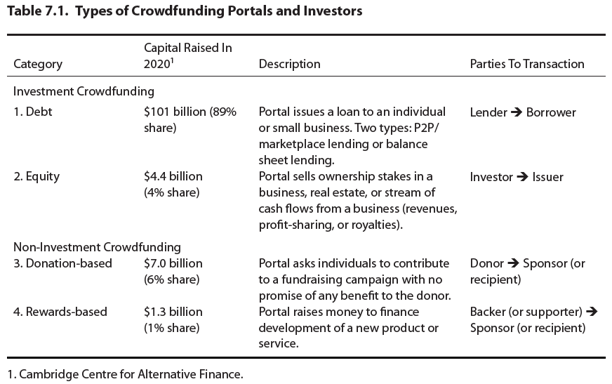
\includegraphics[]{Crowdfunding/figures/TypeOfCroudfunding.png}
    } %end of resizebox
%-----------------------------------------------
% Figure setting: caption and label
%-----------------------------------------------
%\caption{xxxxxxxxxxxxxxxxxxxx}
%\label{fig:ModelIntuition_Graphs}
\end{figure}
%-----------------------------------------------
\vspace{-3mm}




\end{frame} 




%------------------------------------------------

\begin{frame}
\frametitle{Online Lending}

Correia (UGA), Han, and Wang (UIUC) study online loans made through online lenders like \href{https://greendayonline.com/online-loan-application/}{Green Day Online} and compare them to traditional ``storefront'' loans. 
 \vfill 
They find that, even looking at different loans made to \emph{the same borrower}, online loans have \textbf{higher interest rates} and \textbf{higher default rates}
 \vfill 
Not explained by differences in collateral, contract design, or credit score implications 
\vfill 
In addition to within-borrower effects, online lenders face \textbf{negative selection}: worse borrowers are more likely to seek loans online 

\end{frame} 
%----------------------------------------------------  

\begin{frame}{Online vs. Storefront Loans}

\begin{center}
    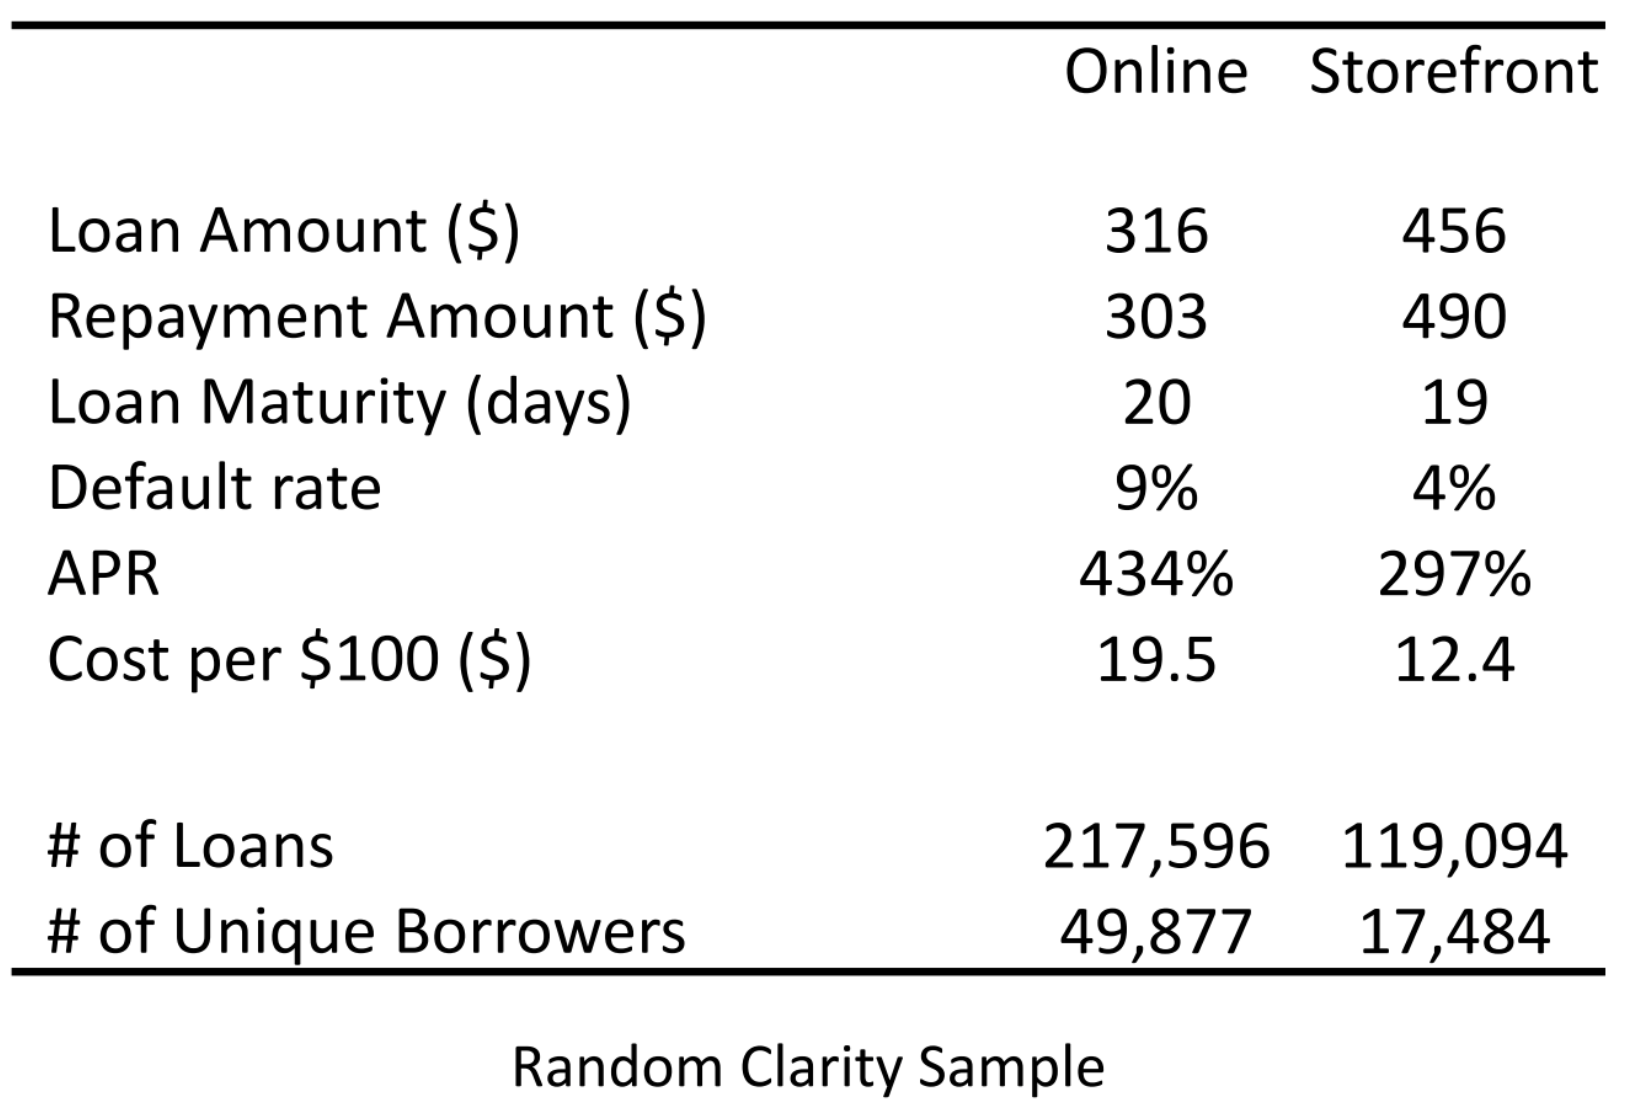
\includegraphics[height = .8\textheight]{Crowdfunding/online_loan_table.png}
\end{center}
    
\end{frame}


%------------------------------------------------

\begin{frame}
\frametitle{Individual vs Business Borrowers}



    \begin{itemize}
        \item Individuals borrow up to \$50,000 and small businesses up to \$500,000 for terms up to 5 years.
        \begin{itemize}
            \item US study (2012-17): avg online borrower is 49 year old with below average credit score borrowing \$8,500 for 3.25 years.
        \end{itemize}
        \item Small businesses have increasingly turned to online lenders to access capital, raising \$43 billion or 43\% of online lending globally in 2020.
    \end{itemize}



\end{frame} 
%----------------------------------------------------  



%------------------------------------------------

\begin{frame}
\frametitle{Comparison of Marketplace Lenders}


%-----------------------------------------------
\begin{figure}[H]
    %\resizebox{\textwidth}{!}{%
    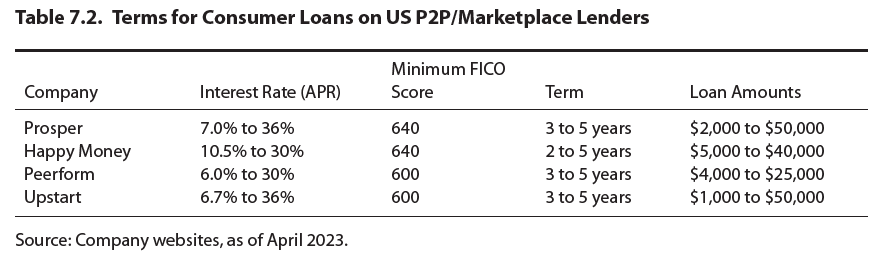
\includegraphics[width = \textwidth]{Crowdfunding/figures/MarketplaceLenders_InterestRate_Fees.png}
%-----------------------------------------------
% Figure setting: caption and label
%-----------------------------------------------
%\caption{xxxxxxxxxxxxxxxxxxxx}
%\label{fig:ModelIntuition_Graphs}
\end{figure}
%-----------------------------------------------



\end{frame} 
%----------------------------------------------------  





%------------------------------------------------

\begin{frame}
\frametitle{Crowdfunding Online Debt Lending}


Institutional investors have leveraged technology to automate the investment process. 
\begin{itemize}
    \item Connect to portal using API, screen and analyze postings in real-time using proprietary computer algorithms (or robots) that make decision to invest or not.
    \item A study of LendingClub found that robot investors outperformed less sophisticated investors. 
\end{itemize}

\medskip 

Does marketplace lending increase financial inclusion?
\begin{itemize}
    \item Some studies find that AI can identify “invisible prime” borrowers who are turned down by traditional lenders due to low FICO scores but are more creditworthy. 
    \item Overall, evidence is mixed, with no clear consensus in the literature on whether AI can meaningfully outperform traditional credit scores. 
\end{itemize}


\end{frame} 
%----------------------------------------------------  




%------------------------------------------------

\begin{frame}
\frametitle{Lendified }


Lendified is fully automated balance sheet lender for small and medium enterprises (SMEs)
\begin{itemize}
    \item Founded in Toronto 2015 by two ex-bankers
    \item Offers loans up to \$150,000 with terms up to 24 months
\end{itemize}

\medskip 


Businesses apply online (under 10 minutes), get an instant decision, and receive funding in 48 hours
\begin{itemize}
    \item Lendified’s software, Judi.ai, connects via API to the applicant’s bank account and generates a cash flow forecast. This forecast is analyzed by a proprietary credit engine to evaluate the ability to finance the loan.
    \item Loan may be collateralized by inventory or accounts receivable to reduce the risk and the cost of borrowing.
    \item Cut loan adjudication costs by 90\%, make decision in minutes, not weeks.
\end{itemize}


\end{frame} 
%----------------------------------------------------  



%----------------------------------------------------  
%----------------------------------------------------  
%\subsection{Equity Crowdfunding}
%----------------------------------------------------  
%----------------------------------------------------  





%------------------------------------------------

\begin{frame}
\frametitle{Crowdfunding Online Equity Issuance}


Regulation of equity crowdfunding: Most start-ups fail so regulators limit how much retail investors may invest in any campaign
\begin{itemize}
    \item SEC's 2024 ``Regulation Crowdfunding'' sets limit on investment at greater of \$2,200 or 5\% of annual income up to \$150,000 (or 10\% of annual income above \$150,000). \href{https://www.sec.gov/education/smallbusiness/exemptofferings/regcrowdfunding}{SEC Regulation on Equity Crowdfunding}
    \item Canada sets cap at CA\$2,500 per deal, or CA\$10,000 if a registered dealer has supplied advice
    \item Other platforms restricted to accredited (high net–worth) investors, such as AngelList
\end{itemize}


\end{frame} 
%----------------------------------------------------  








%------------------------------------------------

%----------------------------------------------------  
%----------------------------------------------------  
%\subsection{Donations and Rewards Crowdfunding}
%----------------------------------------------------  
%----------------------------------------------------  



%------------------------------------------------

\begin{frame}
\frametitle{Donations and Rewards Crowdfunding}


\begin{itemize}
    \item Donation-based crowdfunding ask individuals to contribute to a fundraising campaign with no promise of any benefit to the donor
    \begin{itemize}
        \item Artistic projects, civic projects, charities, medical expenses, or disaster relief.
        \smallskip 
        \item GoFundMe is the world's largest with \$5 billion+ raised.
    \end{itemize}
    \medskip 
    \item Rewards-based crowdfunding raises money to finance the development of a new product or service. 
    \begin{itemize}
        \item Entrepreneur pre-sells a future product to backers (or supporters) who are promised a reward when the project is completed.
        \smallskip
        \item Kickstarter and Indiegogo are biggest in USA.
    \end{itemize}
\end{itemize}



\end{frame} 
%----------------------------------------------------  





%------------------------------------------------

\begin{frame}
\frametitle{Kickstarter Brings Creative Projects to Life}

Support Art, Comics, Crafts, Dance, Design, Fashion, Film \& Video, Food, Games, Journalism, Music, Photography, Publishing, Technology, and Theater.
\begin{itemize}
    \item Since launch in 2009, 23 million people pledged \$7.75 billion of which 250,000+ projects funded (41\% success)
    \item Most successful projects raise less than \$10,000, but close to 800 have raised \$1 million+
    \begin{itemize}
        \item Pebble Time smartwatch (\$20 million), Veronica Mars movie project (\$6 million), Reading Rainbow project (\$5 million).
    \end{itemize}
    \item Creator sets goal and raises funding up to 60 days.
    \item Set up a project page with video and description that explains story behind creative project. Outline the rewards backers will receive when completed.
    \item Monetization: platform (underwriting) fee of 5\% of total funds raised, plus payment processing fee of 3\% + \$0.20 per pledge.
    \item \url{https://www.kickstarter.com/}
\end{itemize}



\end{frame} 
%----------------------------------------------------  



%------------------------------------------------

\begin{frame}
\frametitle{Crowdfunding More Successful in Equity, Donation, and Rewards}



\vspace{-2mm}
%-----------------------------------------------
\begin{figure}[H]
    \resizebox{5.6in}{2.6in}{%
    %\resizebox{\textwidth}{!}{%
    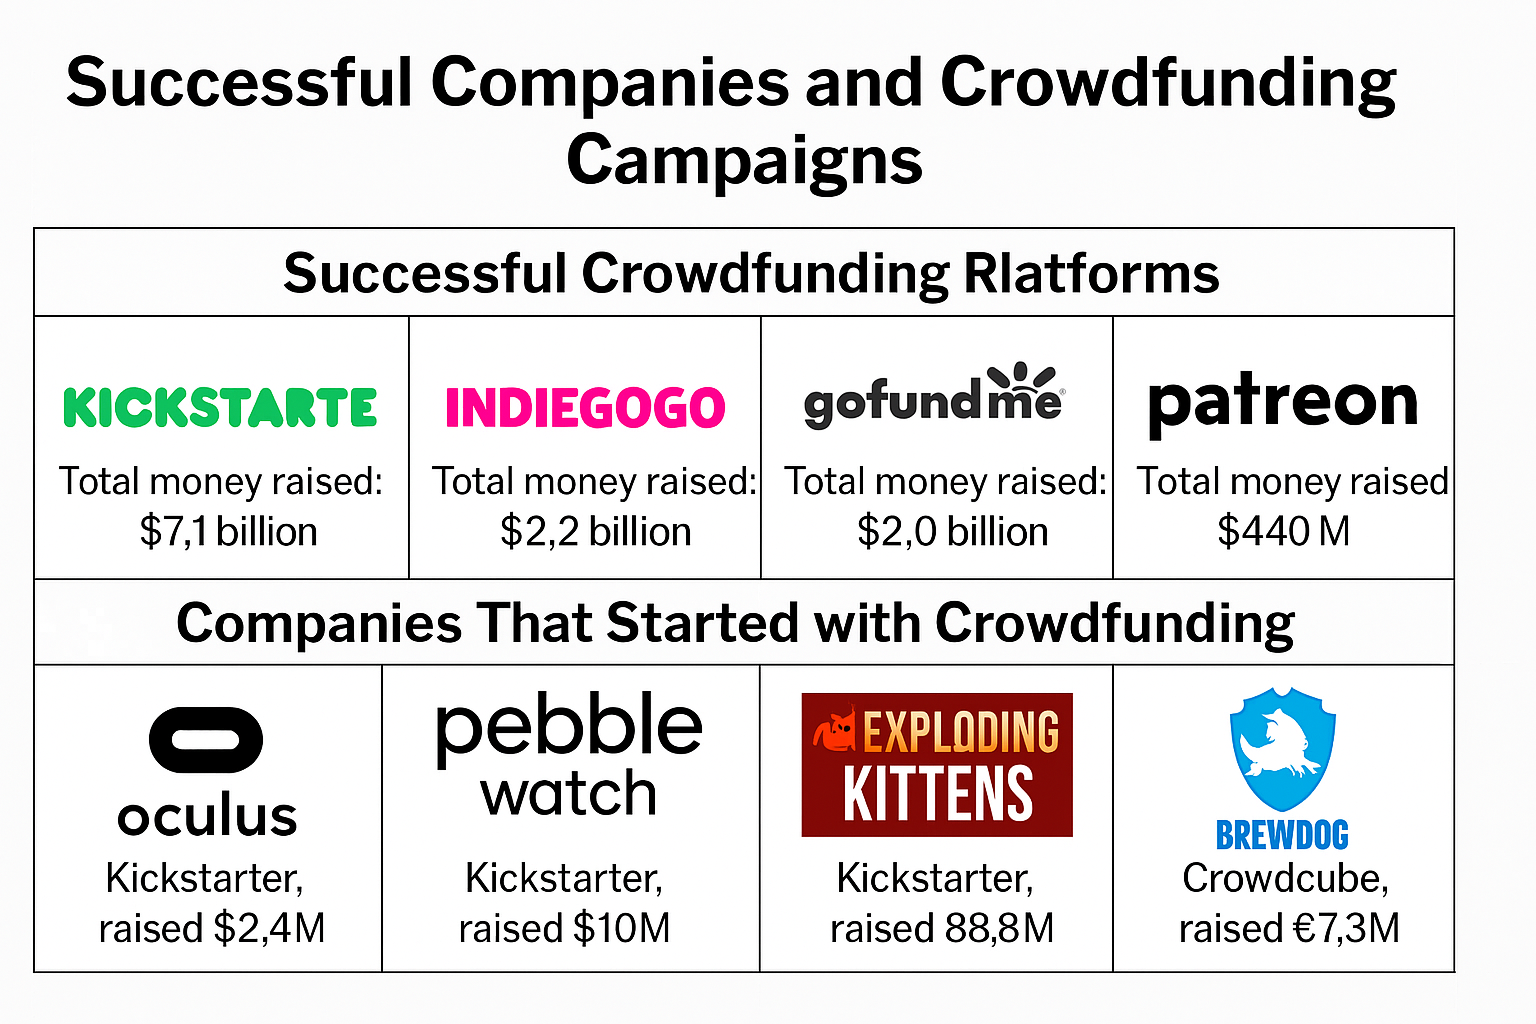
\includegraphics[]{Crowdfunding/figures/SuccessfulCrowdfundingPlatforms_Equity,Donation,Rewards.png}
    } %end of resizebox
%-----------------------------------------------
% Figure setting: caption and label
%-----------------------------------------------
%\caption{xxxxxxxxxxxxxxxxxxxx}
%\label{fig:ModelIntuition_Graphs}
\end{figure}
%-----------------------------------------------
\vspace{-2mm}





\end{frame} 
%----------------------------------------------------  




%----------------------------------------------------  
%----------------------------------------------------  

%\subsection{The Rise and Fall of Crowdfunding Globally}

%----------------------------------------------------  
%---------------------------------------------------- 




%------------------------------------------------

\begin{frame}
\frametitle{The Rise and Fall of Crowdfunding Globally}


Alternative finance grew rapidly over 15 years, reaching US\$419 billion in 2017, with China reaching \textbf{86\% of the global market!} 

\medskip

\begin{itemize}
    \item Widespread fraud, bankruptcies and a regulatory crackdown saw of hundreds of Chinese portals close. Millions of investors lost their life savings.
    \medskip 
    
    \item Fraud case: Ezubao
    \begin{itemize}
        \item founded 2014, became one of China’s largest P2P platforms, raising \$8 billion within 2 years.
        \smallskip 
        \item In early 2016, news outlets reported that 20 people associated with the platform had been arrested for fraud. 
        \smallskip 
        \item Chinese retail investors staged protests in front of police stations, publicly blaming the platform operators and lax regulators for their losses.
    \end{itemize}
\end{itemize}

\end{frame} 
%----------------------------------------------------  




%------------------------------------------------

\begin{frame}
\frametitle{The Rise and Fall of Crowdfunding Globally}

\vspace{-2mm}
By 2020, \$114 billion was raised globally: USA 65\%, Europe 20\%, and China 1\%. 

\begin{itemize}
    \item Alternative finance has raised close to \$1.5 trillion over 2013-2020.
    \item Alternative finance was summarily banned entirely in China. 
    \item Ex-China growth continues. 
\end{itemize}

\vspace{-5mm}
%-----------------------------------------------
\begin{figure}[H]
    \resizebox{5.6in}{1.8in}{%
    %\resizebox{\textwidth}{!}{%
    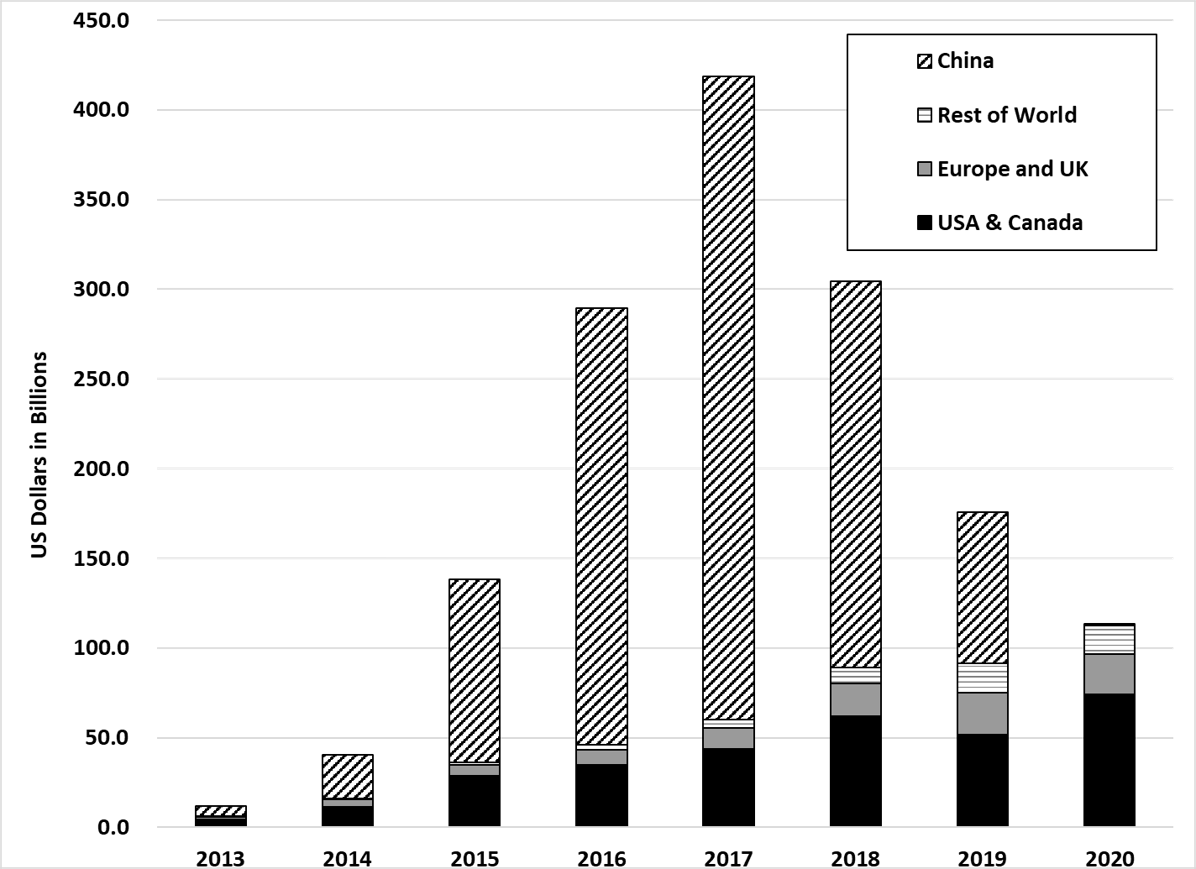
\includegraphics[]{Crowdfunding/figures/Rise&Fall_GlobalCroudfunding.png}
    } %end of resizebox
%-----------------------------------------------
% Figure setting: caption and label
%-----------------------------------------------
%\caption{xxxxxxxxxxxxxxxxxxxx}
%\label{fig:ModelIntuition_Graphs}
\end{figure}
%-----------------------------------------------
\vspace{-4mm}




\end{frame} 
%----------------------------------------------------  



%------------------------------------------------

\begin{frame}
\frametitle{The Rise and Fall of Crowdfunding Globally}

\vspace{-2mm}
Alternative Finance Market Size and Growth
\begin{itemize}
    \item In 2020, debt crowdfunding was 89\% of funding raised, equity 4\%, and non-investment (donation, rewards) 7\%.
\end{itemize}


\vspace{-5mm}
%-----------------------------------------------
\begin{figure}[H]
    \resizebox{5.6in}{2.2in}{%
    %\resizebox{\textwidth}{!}{%
    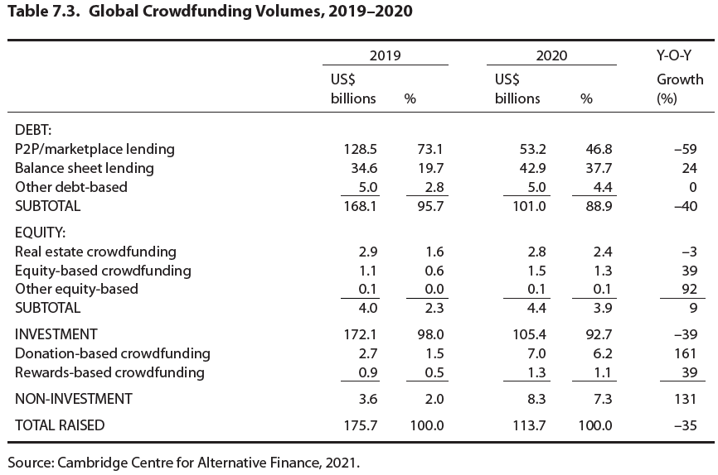
\includegraphics[]{Crowdfunding/figures/GlobalCroudfunding_Type_2019&2020.png}
    } %end of resizebox
%-----------------------------------------------
% Figure setting: caption and label
%-----------------------------------------------
%\caption{xxxxxxxxxxxxxxxxxxxx}
%\label{fig:ModelIntuition_Graphs}
\end{figure}
%-----------------------------------------------
\vspace{-4mm}



\end{frame} 
%----------------------------------------------------  



%------------------------------------------------



%------------------------------------------------


%------------------------------------------------

\begin{frame}
\frametitle{Regulations and Logistics}

Regulation is a high barrier to entry
\begin{itemize}
        \item U.S. crowdfunding platforms are covered by federal and state licensing requirements, consumer protection laws, securities laws, anti-money laundering laws, and national securities association (FINRA) rules.
        \item They must register with the U.S. Securities and Exchange Commission (SEC), become a FINRA member, and meet ongoing reporting and disclosure requirements.
    \end{itemize}

\medskip 

In 2016, the Office of the Comptroller of the Currency (OCC) announced plans to issue a special fintech charter that would allow online portals to be supervised federally and not by states.
\begin{itemize}
    \item Square \textcolor{red}{applied in 2017} and \textcolor{red}{received its charter in 2020}.
    \item SoFi \textcolor{red}{applied in 2017} and \textcolor{red}{received its charter in 2022}.
    \item Many fintechs have not applied, preferring to use banking-as-a-service 
\end{itemize}



\end{frame} 
%----------------------------------------------------  

%---------------------------------------------------- 
%---------------------------------------------------- 
%\subsection{Business Model}
%---------------------------------------------------- 
%---------------------------------------------------- 



%------------------------------------------------

\begin{frame}
\frametitle{How Crowdfunding Portals Make Money}


They charge fees to users on various sides of their multi-sided platforms: (1) Issuers or borrowers on one side; (2) Investors or lenders on the other
 

\medskip 


\begin{itemize}
    \item Sign-up fee: may charge a listing fee regardless of success or failure of campaign
    \item Subscription fee: or charge a monthly or annual fee that allows issuers to run campaigns over a fixed period
    \item Underwriting fee: 1\% to 5\% of any capital raised
    \item Carry percentage / warrants: platform may invest in the campaign and share upside if successful
    \item Payment processing fee: 3\% on payments plus an amount per pledge paid (similar to a credit card issuer)
    \item Management fee: a percentage of assets under management (AUM)
\end{itemize}



\end{frame} 
%----------------------------------------------------  





%------------------------------------------------

\begin{frame}
\frametitle{How Crowdfunding Portals Make Money}


Online lending portals charge fees to both the borrower and the lender:
\begin{itemize}
    \item Loan interest rate: 6\% to 30\% APR, or more
    \item Origination fee: 3.0\% to 6.5\% of amount raised
    \item Late or missed payment fee: specified in the loan contract (called an indenture);
    \begin{itemize}
        \item Example: overdue payment fee equal to 15\% of missing loan payments
    \end{itemize}
    \item Servicing fee: 1\% to 3\% of each payment
    \item Marketing (or Transaction) fee: charge a bank, a hedge fund, or a high net–worth individual a fee to cover the expense of acquiring customers. LendingClub charges banks 1\% to 6\% of the face amount of the loan.
\end{itemize}



\end{frame} 
%----------------------------------------------------  



%------------------------------------------------




%---------------------------------------------------- 
%---------------------------------------------------- 
%\subsection{Crowdfunding Research Findings}
%---------------------------------------------------- 
%---------------------------------------------------- 


%------------------------------------------------

\begin{frame}
\frametitle{Crowdfunding Research Findings: Mixed Evidence}


Competition and Financial Inclusion
\begin{itemize}
    \item Entered markets with fewer bank branches, lower incomes, more minority households, underbanked rural communities, industries with fewer banking relationships,
    \item Entered markets where complaints about bank misconduct are higher, and where banks have pulled back during past economic downturns (including 2008 global financial crisis).
\end{itemize}

\medskip 

Other studies disagree, saying they target borrowers with higher credit scores and education
\begin{itemize}
    \item Online lenders do not target risky or marginal borrowers who have low access to finance, but instead provide credit to borrowers who already have access via banks.
    \item Fintech mortgage lenders process mortgage applications 20\% faster than other lenders but charge a premium interest rate and serve more educated and older borrowers with good access to finance.
\end{itemize}



\end{frame} 
%----------------------------------------------------  




%------------------------------------------------

\begin{frame}
\frametitle{Crowdfunding Research Findings: Mixed Evidence}


Discrimination and Bias in Alternative Finance
\begin{itemize}
    \item Female entrepreneurs represented only 35\% of Kickstarter campaigns but had higher funding success.
    \item Experienced male and female investors show no gender bias when investing in projects. But inexperienced female investors favored female founders.
    \item African American men are significantly less likely than similar white founders to receive equity crowdfunding.
    \item Latinx (Latin American origin) and African American borrowers were charged significantly higher interest rates on online mortgages.
    \item Algorithmic decision-making tools such as machine learning may incorporate bias. When trained on data that itself incorporates human biases based on gender, race, income levels, and other factors.
\end{itemize}



\end{frame} 
%----------------------------------------------------  



%----------------------------------------------------  
%----------------------------------------------------  
%\subsection{Case: LendingClub}
%----------------------------------------------------  
%----------------------------------------------------  



%------------------------------------------------

\begin{frame}
\frametitle{LendingClub's Marketplace Lending Platform}



\vspace{-2mm}
%-----------------------------------------------
\begin{figure}[H]
    \resizebox{4in}{0.8in}{%
    %\resizebox{\textwidth}{!}{%
    
\includegraphics[]{Crowdfunding/figures/LendingClub_Logo.jpeg}
    } %end of resizebox
%-----------------------------------------------
% Figure setting: caption and label
%-----------------------------------------------
%\caption{Insurtech Performance First Year Post-IPO}
%\label{fig:ModelIntuition_Graphs}
\end{figure}
%-----------------------------------------------
\vspace{-2mm}


\vspace{-2mm}
LendingClub is a U.S.-based financial technology company known for launching one of the first major peer-to-peer (P2P) lending platforms in the world. 
\medskip 
\begin{itemize}
    \item Founded in 2006, it began as a marketplace where individual borrowers could access personal loans funded by individual or institutional investors.
    \medskip 
    \item 2007: Becomes the first P2P lender to register its offerings with the SEC
    \medskip 
    \item 2014: Went public on the NYSE, raising \$870 million — one of the largest fintech IPOs
    \medskip 
    \item 2021: Acquired Radius Bank, becoming a fully chartered digital bank — a major pivot from marketplace lending to traditional banking
\end{itemize}


\end{frame} 
%----------------------------------------------------  




%------------------------------------------------

\begin{frame}
\frametitle{LendingClub's Marketplace Lending Platform}


\footnotesize
\begin{columns}[T]
    % Left Column: Years 2007-2015
    \begin{column}{0.48\textwidth}
        \begin{tabular}{rlp{3.5cm}}
            \toprule
            \textbf{Year} & \textbf{Billion} & \textbf{Key Events} \\
            \midrule
            2007 & 0.002 & Launched as Facebook app \\
            2008 & 0.01 & Early P2P lending model \\
            2009 & 0.03 & Shift to direct lending \\
            2010 & 0.2 & Secures major funding \\
            2011 & 0.5 & Institutional investors join \\
            2012 & 1.0 & Expands loan categories \\
            2013 & 2.1 & Prepares for IPO \\
            2014 & 4.3 & Goes public (NYSE: LC) \\
            2015 & 8.4 & Record growth post-IPO \\
            \bottomrule
        \end{tabular}
    \end{column}

    % Right Column: Years 2016-2024
    \begin{column}{0.48\textwidth}
        \begin{tabular}{rlp{3.5cm}}
            \toprule
            \textbf{Year} & \textbf{Billion} & \textbf{Key Events} \\
            \midrule
            2016 & 8.8 & CEO resignation scandal \\
            2017 & 7.9 & Regulatory crackdown \\
            2018 & 10.9 & Acquires Radius Bank \\
            2019 & 12.2 & Peak origination volume \\
            2020 & 4.3 & COVID-19 shutdowns \\
            2021 & 10.4 & Rebound; digital banking push \\
            2022 & 13.1 & steady growth \\
            2023 & 7.4 & Rate hikes slow lending \\
            \bottomrule
        \end{tabular}
    \end{column}
\end{columns}




\end{frame} 
%----------------------------------------------------  







%------------------------------------------------

\begin{frame}
\frametitle{LendingClub's Marketplace Lending Platform}

\vspace{-2mm}
LendingClub was listed on the NYSE in 2014 at \$15.00 per share
\begin{itemize}
    \item LC had originated \$6 billion in loans over 7-years but was still unprofitable.
    \item The stock price rose to \$25.74, then declined steadily.
\end{itemize}



\vspace{-2mm}
%-----------------------------------------------
\begin{figure}[H]
    \resizebox{5in}{2in}{%
    %\resizebox{\textwidth}{!}{%
    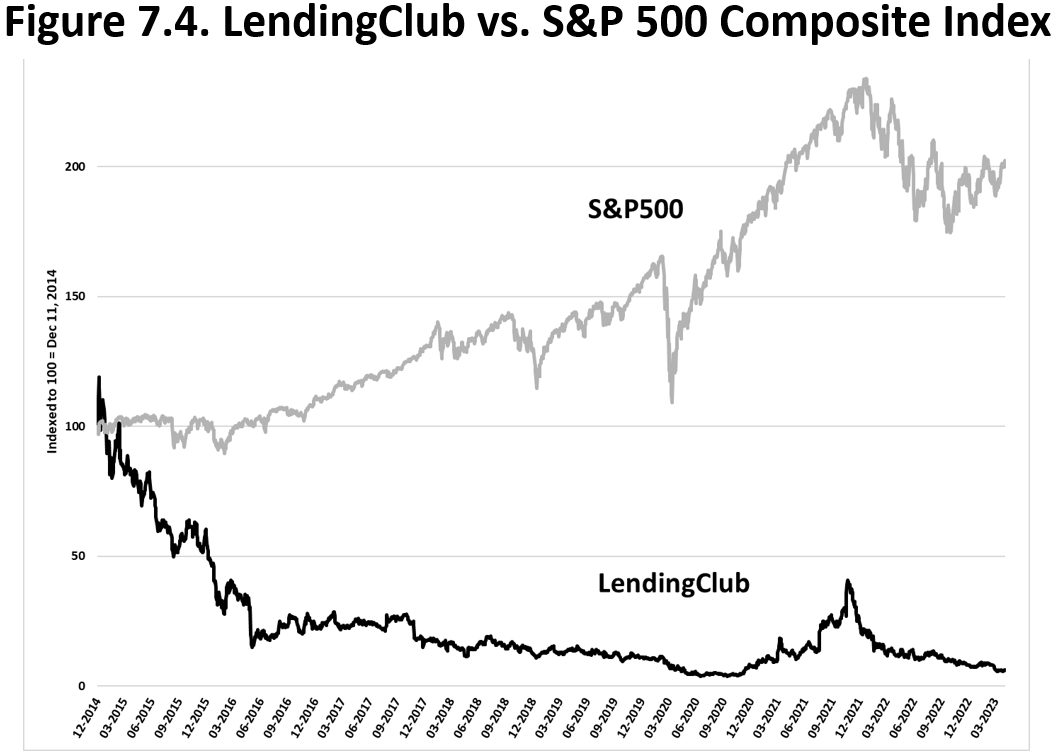
\includegraphics[]{Crowdfunding/figures/LendingClub_vs_S&P500.png}
    } %end of resizebox
%-----------------------------------------------
% Figure setting: caption and label
%-----------------------------------------------
%\caption{Insurtech Performance First Year Post-IPO}
%\label{fig:ModelIntuition_Graphs}
\end{figure}
%-----------------------------------------------
\vspace{-2mm}



\end{frame} 
%----------------------------------------------------  




%----------------------------------------------------  
%----------------------------------------------------  
%\subsection{Case: SoFi}
%----------------------------------------------------  
%----------------------------------------------------  


%------------------------------------------------

\begin{frame}
\frametitle{SoFi’s Evolution from Online Lender to Full-Service Bank}

\vspace{-2mm}
Social Finance (SoFi) was founded as a P2P lender

\begin{itemize}
    \item Started in San Francisco in 2011 by four Stanford business school students who saw gap for alumni to fund MBA students at leading U.S. universities.
    \begin{itemize}
        \item By 2013, SoFi had funded \$200 million in loans to 2,500 undergraduate and graduate students at 100 eligible schools.
        \item SoFi moved away from this base, raising funding from  angels, VCs and banks. They securitized their loan book.
        \item They focused on building relationships with former borrowers (called members) through singles events, wine tastings, career counseling, and home-buying workshops.
    \end{itemize}
\end{itemize}

\medskip 

SoFi has grown to become a one-stop shop for financial services that allows members to borrow, save, spend, invest, and protect their money.
\begin{itemize}
    \item In mid-2021, SoFi went public in a SPAC-related IPO that valued the fintech at \$9 billion.
    \item SoFi was the largest non-bank unsecured consumer lender in the United States.
\end{itemize}



\end{frame} 
%----------------------------------------------------  




%------------------------------------------------

\begin{frame}
\frametitle{SoFi’s Evolution from Online Lender to Full-Service Bank}

\vspace{-2mm}
Despite the success and media attention, SoFi has lost money in its last three fiscal years 

\begin{itemize}
    \item Operating expenses exceed revenues by a large margin
\end{itemize}


\vspace{-2mm}
%-----------------------------------------------
\begin{figure}[H]
    \resizebox{5in}{1.8in}{%
    %\resizebox{\textwidth}{!}{%
    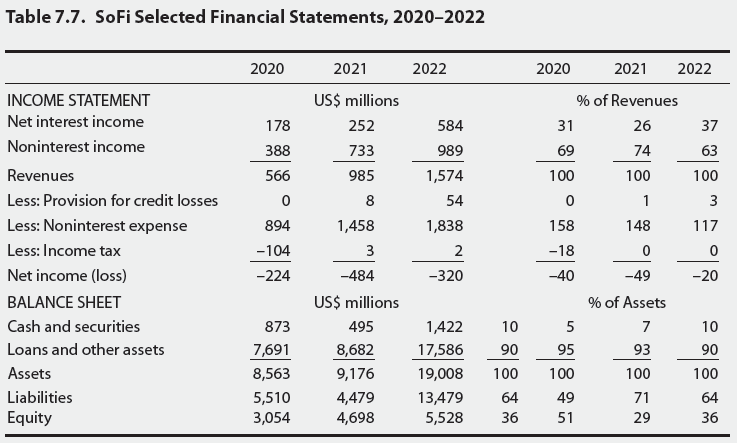
\includegraphics[]{Crowdfunding/figures/Sofi_FinancialStatement_2020To2022.png}
    } %end of resizebox
%-----------------------------------------------
% Figure setting: caption and label
%-----------------------------------------------
%\caption{xxxxxxxxxxxxxxxxxxxx}
%\label{fig:ModelIntuition_Graphs}
\end{figure}
%-----------------------------------------------
\vspace{-4mm}



\end{frame} 
%----------------------------------------------------  




%------------------------------------------------


%----------------------------------------------------  
%----------------------------------------------------  
%----------------------------------------------------  
%----------------------------------------------------

\end{document}